\documentclass[a4paper,USenglish,cleveref,autoref,thm-restate,anonymous]{lipics-v2021}
%This is a template for producing LIPIcs articles. 
%See lipics-manual.pdf for further information.
%for A4 paper format use option "a4paper", for US-letter use option "letterpaper"
%for british hyphenation rules use option "UKenglish", for american hyphenation rules use option "USenglish"
%for section-numbered lemmas etc., use "numberwithinsect"
%for enabling cleveref support, use "cleveref"
%for enabling autoref support, use "autoref"
%for anonymousing the authors (e.g. for double-blind review), add "anonymous"
%for enabling thm-restate support, use "thm-restate"
     
%\graphicspath{{./graphics/}}%helpful if your graphic files are in another directory

\hideLIPIcs 

\ccsdesc{%
Theory of computation $\rightarrow$ 
Design and analysis of algorithms $\rightarrow$ 
Parameterized complexity and exact algorithms $\rightarrow$ 
Fixed parameter tractability}


% TODO 



\bibliographystyle{plainurl}
\newcommand{\citet}[1]{\cite{#1}}
\usepackage{graphicx}
\urlstyle{rm}
\def\UrlFont{\rm}
\usepackage{graphicx} 
\newif\iflong
\newif\ifshort

% comment the below line out for short version
\longtrue

\keywords{parameterized complexity, NLC-width, rank-width, decision trees, partially defined Boolean formulas}

\usepackage{tikz}
\usepackage{booktabs}
\usepackage[noend]{algpseudocode}
\usepackage{algorithm,algorithmicx}
\newcommand{\NULL}{\textnormal{\texttt{nil}}}
\newcommand{\TRUE}{\texttt{TRUE}}
\newcommand{\FALSE}{\texttt{FALSE}}

\algnewcommand\algorithmicinput{\textbf{Input:}}
\algnewcommand\INPUT{\item[\algorithmicinput]}

\algnewcommand\algorithmicoutput{\textbf{Output:}}
\algnewcommand\OUTPUT{\item[\algorithmicoutput]}

% decision trees and parameters
\newcommand{\DTL}{\probfont{DTS}}
\newcommand{\DTLh}{\probfont{DTD}}
\newcommand{\MSS}{\textup{MSS}}
\newcommand{\MNE}{\min_{\#}}
\newcommand{\GIL}{G^+_I}


\newcommand{\inst}{I}
\newcommand{\MIHS}{\probfont{MIHS}}

% \newcommand{\HD}{\delta}
% \newcommand{\MHD}{\delta_{\max}}
%\newcommand{\DMAX}{D_{\max}}

% \newcommand{\GD}{D}
% \newcommand{\IV}{I}

\usepackage{todonotes}
\presetkeys%
    {todonotes}%
    {inline,backgroundcolor=yellow}{}

%table stuff?
\usepackage{booktabs}
\usepackage{multirow}
%\usepackage{floatrow}

\usepackage{amsthm,amsmath,amssymb}
\usepackage{enumerate,verbatim}
\usepackage{xspace}

\usepackage{tikz,tikz-cd}
\usetikzlibrary{arrows,cd,positioning,shapes,patterns}


\usepackage[draft,author=]{fixme}
\fxsetup{theme=color}
%\newcommand{\todo}[1]{\fxerror{#1}}
\newcommand{\warn}[1]{\fxwarning{#1}}
\renewcommand{\note}[1]{\fxnote{#1}}
\newcommand{\nb}[1]{\todo{\scriptsize #1}}



\newcommand{\SB}{\{\,}
\newcommand{\SM}{\;{|}\;}
\newcommand{\SE}{\,\}}
\newcommand{\PP}{\mathcal{P}}
\newcommand{\QQ}{\mathcal{Q}}
\newcommand{\III}{\mathcal{I}}
\newcommand{\SSS}{\mathcal{S}}
\newcommand{\RRR}{\mathcal{R}}
\newcommand{\DDD}{\mathcal{D}}
\newcommand{\FFF}{\mathcal{F}}
\newcommand{\TTT}{\mathcal{T}}
\newcommand{\VVV}{\mathcal{V}}
\newcommand{\XXX}{\mathcal{X}}

\newcommand{\RR}{\mathcal{R}} 

\newcommand{\Z}{\mathbb{Z}}
\newcommand{\Nat}{\mathbb{N}}
\newcommand{\downcl}[2]{D_{#1}(#2)}
\newcommand{\pref}{P_{\leq^V}}
\newcommand{\suff}{S_{\leq^V}}

\newcommand{\bigoh}{\mathcal{O}}
\newcommand{\littleoh}{o}

 
 


\newcommand{\cc}[1]{{\mbox{\textnormal{\textsf{#1}}}}\xspace}  %% Complexity class
\newcommand{\cocc}[1]{{\mbox{\textrm{co}\textnormal{\textsf{#1}}}}\xspace}  %% Complexity class

\newcommand{\integers}{\mathbb{Z}}
\renewcommand{\P}{\cc{P}}
\newcommand{\NP}{\cc{NP}}
\newcommand{\coNP}{\cc{co-NP}}
\newcommand{\FPT}{\cc{FPT}}
\newcommand{\XP}{\cc{XP}}
\newcommand{\Weft}{{\cc{W}}}
\newcommand{\W}[1]{{\Weft}{{\textnormal[#1\textnormal]}}}
\newcommand{\paraNP}{\cc{paraNP}}
\newcommand{\paraNPs}{\cc{pNP}}


\newcommand{\fpt}{fixed-pa\-ra\-me\-ter trac\-ta\-ble\xspace}

\newcommand{\tuple}[1]{\langle{#1}\rangle}  % Tuple
\newcommand{\pn}[1]{\textsc{#1}}
\newcommand{\hy}{\hbox{-}\nobreak\hskip0pt}

%\newcommand{\citet}[1]{\citeauthor{#1}~\shortcite{#1}\xspace}
\newcommand{\nn}{\mathbb{N}}

\newcommand{\bigO}[1]{\ensuremath{{\mathcal O}(#1)}}
\newcommand{\bigOstar}[1]{\ensuremath{{\mathcal O}^*(#1)}}

\newcommand{\probfont}[1]{\textnormal{\textsc{#1}}}

%\newcommand{\stw}{dependency treewidth}



%\newcommand{\RAPROG}{\probfont{Proportionality Graph Allocation}}
\newcommand{\RAENVG}{\probfont{(Locally) Envy-Free Allocation}}
\newcommand{\RAENVGNL}{\probfont{Envy-Free Allocation}}
\newcommand{\RAENVGL}{\probfont{Locally Envy-Free Allocation}}

\newcommand{\EFA}{\textsc{EFA}}
\newcommand{\LEFA}{\textsc{LEFA}}

\newcommand{\FCGENVPROP}{envy-free}
\newcommand{\FCGENV}{locally envy-free}
\newcommand{\FCGPROP}{proportional}

\newcommand{\AT}{T_A}
\newcommand{\RT}{T_R}
\newcommand{\mundef}{\textup{undef}}
\newcommand{\BS}{\textup{BS}}

\newcommand{\RofRT}{R}
\newcommand{\RTBUN}{\textup{BUN}}
\newcommand{\RTVEC}{\vec{b}}
\newcommand{\RTVECSET}{\mathcal{B}}

\newcommand{\rall}{\alpha}
\newcommand{\itf}{\vec{u}}
\newcommand{\new}[1]{}
\newcommand{\valn}{\beta}
\newcommand{\VR}{\RRR}


\newcommand{\prop}[1]{#1}
\newcommand{\noprop}[1]{}
\newcommand{\bunmin}{\alpha_{\min}}
\newcommand{\bunmax}{\alpha_{\max}}
\newcommand{\propmax}{\beta}
\usepackage{boxedminipage}

\newcommand{\MCC}{\probfont{Multicolored Clique}}

\newcommand{\pbDef}[3]{%
\noindent
\begin{center}
\begin{boxedminipage}{0.98 \columnwidth}
#1\\[5pt]
\begin{tabular}{l p{0.70 \columnwidth}}
Input: & #2\\
Question: & #3
\end{tabular}
\end{boxedminipage}
\end{center}
}

\newcommand{\pbDefP}[4]{%
\noindent
\begin{center}
\begin{boxedminipage}{0.98 \columnwidth}
#1\\[5pt]
\begin{tabular}{l p{0.70 \columnwidth}}
Input: & #2\\
Parameter: & #3\\
Question: & #4
\end{tabular}
\end{boxedminipage}
\end{center}
}


\newcommand{\lc}{l}
\newcommand{\rc}{r}

\newcommand{\reaches}{r}


\newcommand{\CCC}{\mathcal{C}}

\newcommand{\ol}[1]{\overline{#1}}
\newcommand{\Card}[1]{|#1|}
\let\phi=\varphi
\let\epsilon=\varepsilon 
\def\hy{\hbox{-}\nobreak\hskip0pt} 
% Name for our encoding and for the whole approach
\newcommand{\enc}{DT\_pb}
\newcommand{\ench}{DT\_hyb}
\newcommand{\slv}{DT\_rec}
% Subsampling strategies
\newcommand{\stratrand}{RandSelect}
\newcommand{\stratlearn}{TreeSelect}
\newcommand{\stratleaf}{LeafSelect}
\newcommand{\stratinc}{MonotonicSelect}
% Feature reduction
\newcommand{\redcon}{\text{FR}}
\newcommand{\redgreedy}	{$\redcon_{\text{greedy}}$}
\newcommand{\redmaxsat}	{$\redcon_{\text{maxsat}}$}
\newcommand{\redrand}	{$\redcon_{\text{rand}}$}
\newcommand{\reddec}	{$\redcon_{\text{back}}$}

% reduction flags
\newcommand{\redinit}{RI}
\newcommand{\redinc}{RC}

\newcommand{\dif}{\text{\specialfont{diff}}}
\newcommand{\dom}{\text{\specialfont{dom}}}
\newcommand{\siz}{\text{\specialfont{size}}}
\newcommand{\solsize}{\text{\specialfont{sol}}}

\newcommand{\parameter}[1]{\text{\normalfont{\sffamily #1}}}
 

\newcommand{\var}{\text{\specialfont{feat}}}


\newcommand{\leaf}{\text{\specialfont{leaf}}}



\newcommand{\specialfont}[1]{{\normalfont\slshape #1}}

\newcommand{\nlcw}{\text{\specialfont{nlcw}}}
\newcommand{\rtw}{\text{\specialfont{rtw}}}
\newcommand{\tw}{\text{\specialfont{tw}}}
\newcommand{\cw}{\text{\specialfont{cw}}}
\newcommand{\rw}{\text{\specialfont{rw}}}
\newcommand{\dep}{\text{\specialfont{dep}}}
\newcommand{\ghtw}{\text{\specialfont{ghtw}}}
\newcommand{\htw}{\text{\specialfont{htw}}}

% DT makros

\newcommand{\SoIF}[1]{I_{#1}}
\newcommand{\SoFF}[1]{F_{#1}}
\newcommand{\anc}{\textit{\textup{anc}}}
\newcommand{\AL}{A}
\newcommand{\thr}{\lambda}
\newcommand{\thres}{\lambda}
\newcommand{\feat}{\text{\specialfont{feat}}}
\newcommand{\reflip}[1]{\textcolor{lipicsGray}{\sffamily\bfseries\upshape\mathversion{bold}\ref{#1}}}
\newcommand{\DTnass}{\tau}

\begin{document}
%\raggedright\pagestyle{empty}\nolinenumbers


  


\title{%Fixed-Parameter Tractability of\\  Learning Small Decision  Trees%
Learning Small Decision Trees for\\ Data of Low Rank-Width
  \iflong
  \\(full paper)
  \fi
}


\author{TODO}{~}{~}{}{}
\authorrunning{~}
\titlerunning{Learning Small Decision Trees for Data of Low Rank-Width}
\maketitle


\begin{abstract}
  We consider the NP-hard problem of finding a smallest decision tree
  representing a given Boolean classification instance (CI), also
  known as a partially defined Boolean function. We show that the
  problem is fixed-parameter tractable when parameterized by the
  rank-width of the given CI. Our algorithm proceeds by dynamic
  programming using an NLC decomposition of the CI, which is obtained
  from the CI's rank-width decomposition.  The key to the algorithm is a
  succinct representation of partial solutions so that each dynamic
  programming step's space and time requirements remain bounded in
  terms of the parameter.
\end{abstract}
 
\newpage
\clearpage
\setcounter{page}{1}

\section{Introduction}
Decision trees have proved to be extremely useful tools for 
describing, classifying, generalizing
data~\cite{Larose05,Murthy98,Quinlan86}. In this paper, we consider
decision trees for {\it classification instances (CIs)}, consisting of
a finite set $E$ of {\it examples} (also called {\it feature vectors})
over a finite set $\feat(E)$ of {\it features}. Each example $e\in E$ is a
function $e:\feat(E)\rightarrow \{0,1\}$ which determines whether the
feature~$f$ is true or false for $e$.  Moreover, $E$ is given as a
partition $E^+ \uplus E^-$ into positive and negative examples. For
instance,  examples could represent medical patients and features
diagnostic tests; a patient is positive or negative corresponding to
whether they have been diagnosed with a certain disease or not. CIs
are also called {\it partially} or {\it incompletely defined Boolean
  functions}, as we can consider the features as Boolean variables,
and examples as  truth assignments that evaluate to 0 (for positive
examples) or 1 (for negative examples). CIs have been studied as a key
concept for the logical analysis of data and in switching theory
\cite{BorosCHIKM11,Boros03,BorosGHIK95,BorosIbarakiMakino03,
  CramaHammerIbaraki88,IbarakiCramaHammer11,Mccluskey65}.


Because of their simplicity, decision trees are particularly
attractive for providing interpretable models of the underlying CI, an
aspect whose importance has been strongly emphasized over the recent
years~\cite{DarwicheHirth20,DoshivelezKim17,GoodmanFlaxman17,Lipton18,Monroe18}. In
this context, one prefers {\it small trees}, as they are easier to
interpret and require fewer tests to make a classification (a decision
tree is smaller than another if it has fewer nodes). Small trees are
also preferred in view of the parsimony principle (Occam’s Razor)
since small trees are expected to generalize better to new
data~\cite{Bessiere09}. However, given a CI $E=E^+ \uplus E^-$ and an
integer $s$, deciding whether $E$ has a decision tree with at most
$s$ nodes is NP-complete~\cite{HyafilRivest76}.


Given this complexity barrier, we propose a fixed-parameter algorithm
for the problem, which exploits the hidden structure of the input CI
$E$. We capture the hidden structure of $E$ in terms small
\emph{rank-width} of the \emph{incidence graph}, which is the
bipartite graph $G(E)$ whose vertices are the examples on one side and
the features on the other, where an example $e$ is adjacent with a
feature $f$ if and only if $e(f)=1$.  Figure~\ref{fig:example} shows a
CI and a smallest decision tree for it, as well as the incidence
graph.  Recall that rank-width is a well-known graph invariant that
generalizes treewidth in the sense that all graphs of bounded
treewidth have bounded rank-width, but there are dense graphs of
bounded rank-width and unbounded treewidth. We denote the rank-width
and the treewidth of a graph $G$ by $\rw(G)$, and $\tw(G)$,
respectively, and refer to $\rw(G(E))$ and $\tw(G(E))$ as the rank-width
and the treewidth of $E$, respectively.

We can state our main algorithmic result as follows
(for a formal statement see \Cref{cor:trac-tw-b}).

\begin{itemize}\em
\item Computing a smallest decision tree for a given CI $E$ is
  fixed-parameter tractable parameterized by the rank-width of $E$.
\end{itemize}


Next, we argue that rank-width is a particularly well-suited and
general choice as a parameter for this problem because of its
robustness and generality.  Borrowing from a similar notion for
propositional CNF formulas \cite{Lewis78}, we define a \emph{renaming}
$r_X(E)$ of a CI $E$ with respect to a set $X\subseteq \feat(E)$ to be
the CI containing all the examples $e_X$ for $e\in E$ with
$e_X(f)=1-e(f)$ if $f\in X$ and $e_X(f)=e(f)$ if $f\notin X$. Clearly,
the size of a smallest decision tree is the same for $E$ and all its
renamings, and a robust parameter should not depend a particular
chosen renaming. Let is define the \emph{renamable rank-width} of $E$
as $\rw^*(G(E))=\min_{X\subseteq \feat(E)}\rw(r_X(G(E)))$ and the
\emph{renamable treewidth} of $E$ as
$\tw^*(G(E))=\min_{X\subseteq \feat(E)}\tw(r_X(G(E)))$.  For two
integer-valued parameters $p$ and $q$, we say that $p$
\emph{dominates} $q$ if every class of instances for which $q$ is
bounded, also $p$ is bounded; $p$ \emph{strictly dominates} $q$ if $p$
dominates $q$ but $q$ does not dominate $p$.  If $p$ and $q$ dominate
each other, they are \emph{domination-equivalent}. The following
statements (formally shown in Propositions~\ref{prop:rw-rrw},
\ref{prop:rw-rtw}, and \ref{prop:rtw-tw}) certify the robustness and
generality of rank-width for the decision tree problem.

\begin{itemize}%\setcounter{enumi}{1}\em 
\item\label{rw-rw*} Rank-width and renamable rank-width are domination-equivalent.
\item Rank-width strictly dominates renamable treewidth.
\item Renamable treewidth strictly dominates treewidth.
\end{itemize}


\begin{figure}[b]
\small
\begin{minipage}{0.33\linewidth}
\centering
\begin{tabular}{@{}c@{~~}c@{~~}c@{~~}c@{~~}c@{}}
$E$  & $f_1$ & $f_2$ & $f_3$ & $f_4$ \\
\midrule
$e_1 \in E^-$ & 0 & 0 &1 & 0   \\
$e_2 \in E^-$ & 0 & 0 &1 & 1   \\
$e_3\in E^-$ & 0 & 1 &1 & 0 \\
$e_4\in E^-$ & 1 & 1 & 0 & 0   \\
$e_5\in E^+$ & 1 & 0 & 0 & 1  \\
$e_6\in E^+$ & 1 & 0 & 1 & 1  \\
\end{tabular}
\end{minipage}%
\begin{minipage}{0.33\linewidth}
\centering
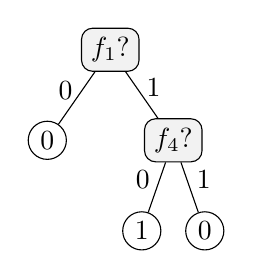
\begin{tikzpicture}[xscale=0.8,yscale=1.15]
\tikzstyle{test} = [draw, rectangle, rounded corners, fill=gray!10]
\tikzstyle{p} = [draw, circle, rounded corners, inner sep=2pt]
\tikzstyle{n} = [draw, circle, rounded corners, inner sep=2pt]
\draw  (0,0) node [test] (A) {$f_1$?}
(1,-1) node [test] (C) {$f_4$?}
(-1,-1) node [n] (B) {0}
(1.5,-2)  node [n] (E) {0}
(0.5,-2)  node [p] (D) {1};
\draw (A) -- (B) node [left,pos=0.35] {0};
\draw (A) -- (C) node [right,pos=0.35] {1};
\draw (C) -- (D) node [left,pos=0.35] {0};
\draw (C) -- (E) node [right,pos=0.35] {1};
\end{tikzpicture}
\end{minipage}%
\begin{minipage}{0.33\linewidth}
\centering
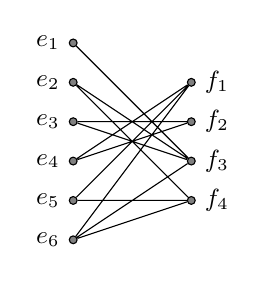
\begin{tikzpicture}[xscale=1.5,yscale=0.5]
\small
\tikzstyle{node} = [draw, circle, rounded corners, fill= gray, inner sep=1pt]
\draw
(0,0) node [node,label=left:$e_1$] (e1) {}
(0,-1) node [node,label=left:$e_2$] (e2) {}
(0,-2) node [node,label=left:$e_3$] (e3) {}
(0,-3) node [node,label=left:$e_4$] (e4) {}
(0,-4) node [node,label=left:$e_5$] (e5) {}
(0,-5) node [node,label=left:$e_6$] (e6) {}
(1,-1) node [node,label=right:$f_1$] (f1) {}
(1,-2) node [node,label=right:$f_2$] (f2) {}
(1,-3) node [node,label=right:$f_3$] (f3) {}
(1,-4) node [node,label=right:$f_4$] (f4) {}
(e1)--(f3) (e2)--(f3) (e2)--(f4) (e3)--(f2) (e3)--(f3) (e4)--(f1) (e4)--(f2) (e5)--(f1) (e5)--(f4) (e6)--(f1) (e6)--(f3) (e6)--(f4);
\end{tikzpicture}
\end{minipage}%
\caption{A CI $E=E^+\uplus E^-$ with six examples and four features (left), a decision tree with~5 nodes that classifies $E$ (middle), the incidence graph $G(E)$ (right).} \label{fig:example}
\end{figure}
  

 

Key to our algorithm are new notions for succinctly representing
decision trees that correspond to subinstances of the incidence graph's
rank decomposition.  Based on that, we can carry out a dynamic
programming (DP) procedure along the rank decomposition. To simplify,
the presentation we will provide the algorithm for NLC-width~\cite{Wanke94} a
well-known parameter that is asymptotically equivalent to rank-width. 
\todo[inline]{I would revert the order and first explain the obstacle
  and how we solve it, and then compare to Bodlaender. How we solve it
could be expanded.}
While the DP approach using rank-width (and other width parameters such
as treewidth) is well understood and can often
be quite easily designed for problems on graphs (or more generally
problems whose solutions can be represented in terms of the graph for
which the rank decomposition is given), the same DP approach can
become rather involved if applied to problems whose solutions have no
or only minor resemblence to the graph for which one is given a rank
decomposition. Probably the most prominent example for this is the
celebrated result by Bodlaender~\cite{Bodlaender96}, where he uses a
DP approach on an approximate tree decomposition to compute the exact
treewidth of a graph; here, the solutions are tree decompositions,
which are complex structures that cannot easily be represented in
terms of the graph. Other prominent examples include a DP approach to
compute the exact treedepth~\cite{DBLP:conf/icalp/ReidlRVS14} or
clique-width~\cite{DBLP:journals/jgaa/EspelageGW03} using an optimal
tree decomposition.  We face a similar problem, since solutions in our
case are decision trees that do not bear any resemblance to the
incidence graph for which we are given the rank decomposition. The
main obstacle to overcome, therefore, is the design of the DP-records
for our DP algorithm. That is, a record for a node $b$ in a rank
decomposition for the incidence graph of $E$ needs to provide a
compact representation of partial solutions, i.e. partial solutions in
the sense that they represent the part of the solution for the whole
instance $E$ that corresponds to the sub-instance induced by all
features and examples contained in the subtree of the rank
decomposition rooted at the current node $b$. We overcome this
obstacle in Section~\ref{sec:twfpt}, where we also provide intuitive
descriptions and motivation for the definition of the records
(Subsection~\ref{ssec:mainideas}). Along the way, we also introduce
various novel notions to deal with DTs such as feature relabellings,
redundancy, contractions and reductions that we believe to be
interesting in their own right.

\ifshort
{\it The full proof of statements marked with $(\star)$ can be found  in the full version of this paper.}
\fi

\todo[inline]{add a brief related work paragraph, mentioning the
  AAAI'21 paper?}


\section{Preliminaries}\label{chap:prelims}

\subsection{Parameterized Complexity}
We give some basic definitions of parameterized complexity and refer
for a more in-depth treatment to other sources
\cite{CyganFKLMPPS15,DowneyFellows13}. Parameterized complexity
considers problems in a two-dimensional
setting, where a problem instance is a pair $(I,k)$, where $I$ is the
main part and~$k$ is the parameter. A parameterized problem is {\it
  fixed-parameter tractable} if there exists a computable function $f$
such that instances $(I,k)$ can be solved in time $f(k) \|I\|^{O(1)}$.

\subsection{Graphs and NLC-width}

We will assume that the reader is familiar with basic graph theory (see, e.g. \cite{BangjensenGutin09,Diestel00}).  We
consider (vertex and edge labelled) undirected graphs. Let $G=(V,E)$
be an undirected graph. We write $V(G)=V$ and $E(G)=E$ for the sets of
vertices and edges of $G$, respectively. We denote an edge between $u
\in V$ and $v \in V$ as $\{u,v\}$. For a set $V' \subseteq V$ of
vertices we let $G[V']$ denote the graph induced by the vertices in
$V'$, i.e. $G[V']$ has vertex set $V'$ and edge set $E \cap \SB
\{u,v\} \SM u,v \in V' \SE$ and we let $G - V'$ denote the graph $G[V
\setminus V']$. For a set $E' \subseteq E$ of edges we let denote
$G-E'$ the graph with vertex set $V$ and edge set $E\setminus E'$.

\newcommand{\lab}{\lambda}

A \emph{$k$-graph} is a pair $(G,\lab)$, where
$G=(V,E)$ is an undirected graph and $\lab : V \rightarrow [k]$ is
a \emph{vertex label mapping} that labels every vertex $v \in V$ with
a label $\lab(v)$ from $[k]$. We call the $k$-graph consisting of exactly one vertex $v$ (say,
labeled by $i$) an \emph{initial $k$-graph} and denote it by $i(v)$.

Node label control-width (\emph{NLC-width}) is a graph parameter, defined as
follows~\cite{Wanke94}: let $k \in \mathbb{N}$ be a positive
integer. A \emph{$k$-NLC-expression tree} of a graph $G=(V,E)$ is a subcubic tree
$B$, where every node $b$ of $B$ is associated with a $k$-graph (denoted by
$(G_b,\lab_b)$), such that:
\begin{enumerate}
\item Every leaf represents an initial $k$-graph $i(v)$ with $i \in
  [k]$ and $v \in V$.
\item Every non-leaf node $b$ with one child $c$ is a \emph{relabelling node}
  and is associated with a relabelling function $R_b:[k] \to
  [k]$. Moreover, $G_b$ is obtained from $G_c$ after relabelling all
  vertices of $G_c$ with label $i$ to label $R_b(i)$ for every $i \in [k]$.
\item Every non-leaf node $b$ with two children, i.e., a left child
  $l$ and a right child $r$, is a
  \emph{join node} and is associated with a \emph{join matrix}, i.e.,
  a binary $k\times k$ matrix
  $M_b$. Moreover, $(G_b,\lab_b)$ is obtained from the disjoint union of
  $(G_{l},\lab_l)$ and $(G_{r},\lab_r)$ after adding an edge from all vertices
  labeled $i$ in $G_{l}$ to all vertices labeled $j$ in $G_{r}$ whenever $M_b[i,j]=1$.
\item $G$ is equal to the $G_r$ for the root node $r$ of $B$.
\end{enumerate}

The NLC-width of a graph~$G$, denoted by~$\nlcw(G)$, is the
minimum~$k$ for which~$G$ has a $k$-NLC-expression tree.
A $k$-NLC-expression tree is {\it nice} if every relabelling node has
a relabelling function $R:[k] \to [k]$ such that for some $i,j \in
[k]$, $R(i)=j$ and $R(\ell)=\ell$ for all $\ell \in [k] \setminus
\{i\}$. Clearly, given a $k$-NLC-expression tree, a nice
$k$-NLC-expression tree can be found in polynomial time; simply replace
every relabelling node (that relabels more than one label at a time)
by a sequence of relabelling nodes.

Let~$b$ be a node in a $k$-NLC-expression tree of a graph~$G$.
We denote by $V_b$ the set of vertices of $G_b$.
%KD: Possibly wnat to prove this/provide a reference.
By the definition of a $k$-NLC-expression tree, if $u,v \in V_b$ have
the same label in $(G_b,\lab_b)$ and $w \in V(G) \setminus V_b$, then~$u$ is adjacent to~$w$ in $G$ if and only if~$v$ is.

%KD: TODO: Compare to clique-width/rank-width.
Computing the NLC-width of a graph is NP-hard~\cite{GurskiWanke05}.
However, it is sufficient to use the algorithm of Oum and Seymour~\cite{OumSeymour06}, which returns a $c$-expression for some $c\leq 2^{3\cw(G)+2}-1$ in $O(n^9\log n)$ time, or the later improvements of Oum~\cite{Oum08} and Hlin\v{e}n\'y and Oum~\cite{HlinenyOum08} that provide cubic-time algorithms which yield a $c$-expression for some $c\leq 8^{\cw(G)}-1$ and $c\leq 2^{\cw(G)+1}-1$, respectively.\todo{should it be $\nlcw$, or should we define $\cw$ and say it's approximation? KD: Could adjust the formulas so that they have the correct ratio for ncl-width rather than clique-width}

\begin{proposition}\label{pro:computeNLC}
  Let $G$ be a graph and $\omega$ an integer. Then, there is a
  linear-time fpt-algorithm (parameterized by $\omega$) either
  correctly concludes that $G$ has NLC-width larger than $\omega$ or
  outputs an $f(\omega)$-NLC-expression tree for $G$.
\end{proposition}

\subsection{Classification Problems}

\newcommand{\GD}{D}
%\newcommand{\Z}{\mathbb{Z}}

An {\it example} $e$ is a function $e:\feat(e) \rightarrow \{0,1\}$ defined
on a finite set $\feat(e)$ of {\it features}. For a set $E$ of
examples, we put $\feat(E)=\bigcup_{e\in E} \feat(e)$. We say that two
examples $e_1,e_2$ {\it agree} on a feature $f$ if $f \in \feat(e_1)$,
$f\in \feat(e_2)$ and $e_1(f)=e_2(f)$. If $f \in \feat(e_1)$, $f \in
\feat(e_2)$ but $e_1(f)\neq e_2(f)$, we say that the examples {\it
  disagree on $f$}.

A {\it classification instance (CI)} (also called a {\it partially
  defined Boolean function}\ \cite{IbarakiCramaHammer11})
$E=E^+ \uplus E^-$ is the disjoint union of two sets of examples,
where for all $e_1,e_2\in E$ we have $\feat(e_1)=\feat(e_2)$. The
examples in $E^+$ are said to be {\it positive}; the examples in $E^-$
are said to be {\it negative}.  A set $X$ of examples is {\it uniform}
if $X\subseteq E^+$ or $X \subseteq E^-$; otherwise $X$ is {\it
  non-uniform}. 
 
Given a CI $E$, a subset $F\subseteq \feat(E)$ is a {\it support set}
of $E$ if any two examples $e_1\in E^+$ and $e_2\in E^-$ disagree in
at least one feature of $F$.  Finding a smallest support set, denoted
by $\MSS(E)$, for a classification instance $E$ is an NP-hard
task~\cite[Theorem 12.2]{IbarakiCramaHammer11}.
 
We define the {\it incidence graph} of $E$, denoted by $G(E)$, as
the bipartite graph with partition $(E, \feat(E))$ having an edge
between an example $e \in E$ and a feature $f\in \feat(e)$ if
$f(e)=1$.



\subsection{Decision Trees}

A \emph{decision tree} (DT) is a rooted binary tree $T$ with vertex set
$V(T)$ and edge set $A(T)$ such that each leaf node is either a
\emph{positive} or a \emph{negative} leaf and the following holds for
each non-leaf $t$ of $T$:
\begin{itemize}
\item $t$ is labeled with a feature denoted by $\feat_T(t)$ or simply
  $\feat(t)$ if $T$ is clear from the context,
\item $t$ has 2 children, i.e., a left child and a right child.
\end{itemize}
We write $\feat(T)=\SB \feat(t) \SM t \in V(T) \SE$ for the set
of all features used by $T$. The size of $T$ is its number of nodes, i.e. $|V(T)|$. 

Let $T$ be a DT. We say that a node $t_A$
is a \emph{left (right) ancestor} of $t$ if $t$ is contained in the
subtree of $T$ rooted at the left (right) child of $t_A$. We denote by
$\anc_T^L(t)$ ($\anc_T^R(t)$), or simply $\anc^L(t)$ ($\anc^R(t)$) if
$T$ is clear from the context, the set of all left (right) ancestors of $t$ in
$T$. We denote by $\anc(t)$ the set of all \emph{ancestors} of $t$ in
$T$, i.e., $\anc(t)=\anc^L(t)\cup\anc^R(t)$.

Let $E$ be a CI and let $T$ be a DT with
$\feat(T)\subseteq \feat(E)$.
For each node $t$ of $T$, we denote by $\DTnass_t$ the partial
feature assignment $\DTnass_t : \feat(\anc(t)) \rightarrow \{0,1\}$
defined by setting $\DTnass_t(f)=0$ if $f \in \feat(\anc^L(t))$ and $\DTnass_t(f)=1$ if $f \in
\feat(\anc^R(t))$. We denote by $E_T(t)$, or simply $E(t)$ if $T$ is
clear from the context, the set $E[\DTnass(t)]$ of examples, where
$E[\DTnass(t)]$ is the set of all examples $e$ in $E$ with
$e(f)=\DTnass_t(f)$ for every feature $f \in \anc(t)$.
We say that $T$ \emph{classifies} an example $e\in E$ if $e$ is a positive (negative)
example and $e\in E_T(l)$ for a positive (negative) leaf $l$ of
$T$. We say that $T$ \emph{is a DT for $E$} if $T$
classifies all examples in $E$.
See Figure~\ref{fig:example} for an illustration of a CI, its incidence graph, and a DT that classifies $E$.

We will consider the following optimisation problem.

\pbDef{\probfont{Minimum Decision Tree Size} (\DTL)}{A CI $E$.}{Find a
  DT of smallest size that classifies $E$.}

We now give some simple auxiliary lemmas that are required by our algorithm.

\begin{lemma}\label{lem:enum-dt-fund}
  Let $A$ be a set of features and $a=|A|$. Then, the number of DTs of
  size at most $s$ that use only features in $A$ is at most $a^{2s+1}$
  and those can be enumerated in $\bigoh(a^{2s+1})$ time.
\end{lemma}
\begin{proof}
  We start by counting the number of trees $T$ with $n$ nodes that can
  potentially underlie a DT with $n$ nodes. Note that there is
  one-to-one correspondence between trees $T$ that underlie a DT with
  $n$ nodes and unlabelled rooted ordered binary trees with $n$ nodes
  (where ordered refers to an ordering of the at most $2$ child
  nodes). Since it is known that the number of unlabelled rooted
  ordered binary trees with $n$ nodes is equal to the $n$-th Catalan
  number $C_n$ and that those trees can be enumerated in $\bigoh(C_n)$
  time~\cite{stanley2015catalan}, we already obtain that we can
  enumerate all of the at most $C_n$ possible trees $T$ underlying a
  DT of size $n$ in $\bigoh(C_n)$ time. Therefore, there are at most
  $sC_{s}$ possible trees of size at most $s$ that can underlie a DT
  with at most $s$ nodes and those can be enumerated in
  $\bigoh(sC_{s})$ time. It now remains to bound the number of
  possible feature assignments $\feat(f)$ for these trees as well as
  the number of possibilities for the leave nodes that can be either
  labelled positive or negative. Since we can assume that $a\geq 2$,
  we obtain that the number of possible feature assignments (and
  labellings of leaf-nodes) of a tree $T$ with $n$ nodes is at most
  $a^n$. Taking everything together, we obtain that there are at most
  $sC_sa^s \leq s4^sa^s \leq a^{2s+1}$ many DTs of size at most $s$
  using only features in $A$ and those can be enumerated in
  $\bigoh(a^{2s+1})$ time.
\end{proof}

\begin{lemma}\label{lem:enum-dt}
  Let $A$ be a set of binary features of size $a$. There are at most
  $a^{2^{a+1}+3}$ inclusion-wise minimal DTs using only features in
  $A$ and these can be enumerated in $\bigoh(a^{2^{a+1}+3})$ time.
\end{lemma}
\begin{proof}
  Note that an inclusion-wise minimal DT $T$ that uses only features in
  $A$ has at most $2^a+1$ nodes; this is because every feature appears
  at most once on every path $T$. Therefore, we obtain from
  Lemma~\ref{lem:enum-dt-fund} that the number of choices for $T$ is at
  most $a^{2(2^a+1)+1}=a^{2^{a+1}+3}$.
\end{proof}

\newcommand{\NO}{\textbf{NO}}
\newcommand{\TsmDT}{(2^{|E|})^{4|E|-1}}

% \begin{lemma}\label{lem:comsmallDT}
%   Let $E$ be a binary CI. Then one can decide whether $E$ has a DT and
%   if so output a DT of minimum size for $E$ in time $\bigoh(\TsmDT)$.
% \end{lemma}

% \begin{proof}
%   Note first that $|\feat(E)|\leq 2^{|E|}$ since we can assume that $E$
%   does not contain two equivalent features. Moreover, $E$ has a DT if
%   and only if $\feat(E)$ is a support set, which can be checked in time
%   $\bigoh(|E|^2|\feat(E)|)$ by checking, for every pair of positive and
%   negative examples in $E$, whether there is a feature that
%   distinguishes them. If this is not the case, we output \NO{}, so
%   assume that $E$ has a DT. Note that any inclusion-wise minimal DT for
%   $E$ has at most $|E|$ leaves and therefore size at most $2|E|-1$. We
%   can therefore employ Lemma~\ref{lem:enum-dt-fund} to enumerate all
%   inclusion-wise minimal potential DTs for $E$ in time
%   $\bigoh((2^{|E|})^{2(2|E|-1)+1}) \in \bigoh(\TsmDT)$. For every such
%   tree we then check whether it is indeed a DT for $E$ and return a DT
%   for $E$ of minimum size found during this process.
% \end{proof}

\newcommand{\exam}{\text{\specialfont{exam}}}







\section{An Algorithm for Rank-width}\label{sec:twfpt}

\newcommand{\afs}{\textup{TF}}
\newcommand{\afsF}{\textup{TF}_F}
\newcommand{\afsP}{\textup{TF}_P}
\newcommand{\addF}{\oplus}

In this section, we show that \DTL{} parameterized by the rank-width of
the incidence graph of the classification instance is fixed-parameter
tractable. To simplify the proof and its description, we will provide
the result for NLC-width. Because of Proposition~\ref{pro:computeNLC},
it suffices to show the result for the case that we are provided with
an $k$-NLC-expression tree.
\begin{theorem}\label{the:trac-nlcw-b-td} 
  Let $E$ be a CI and let $B$ be a $k$-NLC-expression tree for
  $G(E)$. Then, finding a DT of smallest size that classifies $E$ is
  fixed-parameter tractable parameterized by $k$.
\end{theorem}

\begin{corollary}\label{cor:trac-tw-b}
  \DTL{} is fixed-parameter tractable parameterized by NLC-width.
\end{corollary}

The remainder of this section is devoted to a proof of
Theorem~\ref{the:trac-nlcw-b-td}.
In principle, we will use a dynamic programming algorithm along the
$k$-NLC-expression tree $B$ of $G(E)$ that computes a set $\RRR(b)$
of valid records
for every node $b$ of $B$ in a bottom-up (leaf-to-root) manner.
The crucial part will be the correct definition of the records. To
simplify the presentation, we will write $\feat(b)$, $\exam(b)$, and
$E_b$ for the sets $\feat(E)\cap V_b$, $\exam(b) \cap V_b$, and the
subinstance of $E$ induced by the features in $\feat(b)$ and the
examples in $\exam(b)$. We will also call the features and examples of
$E_b$ \emph{old} and we will call all other features and examples in
$E$ \emph{novel}.

\subsection{Informal Description of the Algorithm} \label{ssec:mainideas}

Here, we will informally describe the main ideas behind the definition
of the records for a node $b$ of $B$. Intuitively, a (valid) record for
$b$ will represent a compact representation of an equivalence class of
solutions (DTs) for the whole instance from the perspective of the
subinstance $E_b$.
Therefore, to illustrate the main ideas and
motivations for the later definition
of our records, we need to understand how a solution for the whole
instance, i.e., a DT $T$ that classifies $E$, behaves from the
perspective of the subinstance $E_b$ and what is the information that one
needs to store about $T$.

We start by analysing the role of novel\todo{E: Is it clear what "novel" means? Would it be better to clarify that we mean feature not in $G_b$ when we use it for the first time.}
features used by the nodes in $T$. In particular, let $f$ be a novel feature used by
$T$ and let $e \in \exam(b)$ be an old example. Then, because $B$ is a
$k$-NLC expression tree for $G(E)$ the value $e(f)$ of $f$ for $e$ only
depends on the current label $\lab_b(e)$ of the example $e$ in
$(G_b,\lab_b)$. Therefore, the role of $f$ (and consequently the role
of all novel features) w.r.t. the old examples
in $\exam(b)$ can be described by the set of labels $L \subseteq [k]$
such that $e(f)=1$ if and only if $\lab_b(e)\in L$. This allows us to
replace every novel feature $f$ in $T$ with a so-called future feature $f_L$,
whose behaviour towards the old examples is completely described by the
set $L \subseteq [k]$ of labels, i.e., $e(f_L)=1$ if and only if
$\lab_b(e)\in L$ for every $e \in \exam(b)$.

Let $T^1$ be the tree
obtained from $T$ after replacing all novel features by their
corresponding future features; we will later introduce so-called feature relabellings that will
allow us to relabel features of a DT in a very general manner. Then, $T^1$ is still a DT for
$\exam(b)$ and moreover the future features now act as placeholders
for the novel features and can be replaced later on during the
algorithm. Crucially, we can now also potentially greatly reduce the size
of $T^1$. This is because instead of keeping track of the arbitrarily
many novel features in $T$, we now only need to keep track of the at
most $2^k$ future features (one for every $L \subseteq [k]$).

In
particular, consider a node $t$ of $T^1$ with $\feat(t)=f_L$ for some
set $L\subseteq [k]$ of labels and let $\AL_{T^1}(t)$ be the set of \emph{filtered
labels} (see the next subsection for a formal definition of
$\AL_{T^1}(t)$). Informally, $\AL(t)$ is the set of all labels $\ell
\in [k]$ such that all examples $e\in \exam(b)$ with label $\ell$ would end up at $t$,
if only the effect of the future features on the path from the root of
$T^1$ to $t$ is considered. Then, we say that $t$ is
\emph{left (right) redundant} in $T^1$ if $\AL_{T^1}(t) \subseteq
L'$ ($\AL_{T^1}(t)\subseteq \overline{L'}$). Intuitively, $t$ is left (right) redundant if all
examples that can reach $t$ (considering the influence of the future
features only) end up in the left (right) child of $t$; and therefore
the other child of $t$ is redundant because it will never receive any
examples. To make use of this fact (and to remove redundant nodes) we
will define the following left (right) contraction operation for left
(right) redundant nodes in
a DT. Let $D$ be a DT and $d \in V(D)$ be an inner node of
$D$ with left child $\ell$, right child $r$, and parent $p$.
We say that $D'$ is obtained from $D$ after
\emph{left (right) contracting $d$} if $D'$ is the DT
obtained from $D$ after removing $d$ together with all nodes in $D_r$ ($D_\ell$)
and adding the edge between $p$ and $\ell$ ($r$); if $d$ has no parent then no
edge is added. Therefore, if $t$ is left (right) redundant in $T^1$ we
can left (right) contract $t$ in $T^1$ without changing the behaviour of
$T^1$ towards the old examples in $\exam(b)$.

Let $T^2$ be the tree obtained from $T^1$ after left (right)
contracting every left (right) redundant node $t$ assigned to a future feature.
Note that $T^2$ is still a DT for $\exam(b)$ (for a formal proof see~Observation~\ref{obs:dttred}) . Moreover, it is easy to
see (and will be shown formally in~Observation~\ref{obs:DTSsize}) that any
root-to-leaf path of $T^2$ contains at most $k$ nodes assigned to
future features. We will later call $T^2$ a DT template for $b$.

Let us now consider the role of the old features used in $T^2$ and in particular
what information we need to store about the structure (distribution) of those
features in $T^2$. Note that if we have a record at node $b$, then we
can assume that we already verified that the record can be used to
classify all old examples correctly. Therefore, we only need to store
sufficient information about how the structure of the old features
effects how the record can be extended when novel examples (and features) are added to the subinstance. In other
words, we only need to know how the structure of the old features in
$T^2$ effects the novel examples. 
In particular, let $f$ be an old feature used by $T^2$ and let $e \in
E\setminus \exam(b)$ be a novel example.
Because $B$ is a $k$-NLC expression tree for $G(E)$ the value of $e(f)$ only
depends on the current label $\lab_b(f)$ of the feature $f$ in
$(G_b,\lab_b)$. Therefore, the role of $f$ (and consequently the role
of all old features) w.r.t. to novel examples
can be described by the label of the old feature in $(G_b,\lab_b)$. This allows us to
replace every old feature $f$ in $T^2$ with a so-called forgotten feature $f_l$,
that will behave toward all novel examples in the same manner as every
old feature $f\in \feat(b)$ with label $l$.

Let $T^3$ be obtained from $T^2$ by relabelling every old feature into
its corresponding forgotten feature. Then, $T^3$ behaves in the same
manner as $T^2$ with respect to all novel examples. Moreover, like
$T^1$, also $T^3$ now contains potentially many nodes that are
redundant with respect to their behavior towards novel examples; in
$T^1$ the nodes were redundant concerning their behaviour towards old
examples. To reduce $T^3$, we say that a node $t$ of $T^3$ assigned to
some forgotten feature $f_l$ is left (right) redundant if $t$ has a left
(right) ancestor $t_A$ that is assigned to the same forgotten feature
as $t$. Similarly to before, we can now left (right) contract every
left (right) redundant node in $T^3$ without changing the behaviour of
$T^3$ towards the novel examples.

Let $T^4$ be obtained from $T^3$ after left (right) contracting all
left (right) redundant nodes. Note that every-root-to-leaf path of
$T^4$ can now contain at most $k$ future features and at most $k$
forgotten features, which implies that $T^4$ has bounded height and
therefore also bounded size. $T^4$ is what we will later
call a DT skeleton for $b$ and it contains all the information about
the structure of $T$ that we need to keep in the record corresponding
to $T$. In particular, the record corresponding to $T$ will be the
pair $(T^4,s)$, where $s$ is the number of nodes assigned to forgotten
features in $T^3$ that we have removed to obtained $T^4$, i.e.,
$s=V(T^4)\setminus V(T^3)$. Moreover, informally, we say that such a record is
valid if $s$ is the smallest number such that there is a DT template
for $b$ that reduces to $T^4$ (in the same manner that $T^2$ reduced
to $T^4$). This completes the description of the main ideas behind our records and
we are now ready to provide formal definitions and proofs.



\subsection{Formal Definition of Records and Preliminary Results}

In the following, let $E$ be a CI and let $B$ be a $k$-NLC-expression
tree for $G(E)$. 
% We denote by $\feat(b)$ the set $V_b\cap \feat(E)$ of
% features in $V_b$ and by $\exam(b)$ the set $V_b\cap E$ of examples in
% $V_b$. 
Consider a node $b$ of $B$. 
Let $L$ be a set of labels (usually $L=[k]$). For a subset
$L'\subseteq L$, we denote by $\overline{L'}$ the set $L\setminus L'$.
For a label $\ell \in L$, we introduce a new feature $f_\ell$, which we
will call a \emph{forgotten feature}.
%Informally, forgotten
%features will be used to replace real features in a DT for $b$is that
Moreover, for a subset $L'
\subseteq L$ of labels, we introduce a new feature $f_{L'}$, which we
call an \emph{future (or introduce) feature}. Let $\SoFF{L}=\SB f_\ell \SM \ell \in L\SE$ be the
set of all forgotten features and let $\SoIF{L}=\SB f_{L'} \SM L' \subseteq
L\SE$ be the set of all future features w.r.t. $L$. To distinguish
features in $\feat(E)$ from forgotten and future features, we will
sometimes refer to them as \emph{real features}.

Let $T$ be a DT and $t \in V(T)$ be an inner node of
$T$ with left child $l$, right child $r$, and parent $p$.
We say that $T'$ is obtained from $T$ after
\emph{left (right) contracting $t$} if $T'$ is the DT
obtained from $T$ after removing $t$ together with all nodes in $T_r$ ($T_\ell$)
and adding the edge between $p$ and $l$ ($r$); if $t$ has no parent then no
edge is added.
% Let $T$ be a DT and $t \in V(T)$. We say that a node $t_A$
% is a \emph{left (right) ancestor} of $t$ if $t$ is contained in the
% subtree of $T$ rooted at the left (right) child of $t_A$. We denote by
% $\anc_T^L(t)$ ($\anc_T^R(t)$), or simply $\anc^L(t)$ ($\anc^R(t)$) if
% $T$ is clear from the context, the set of all left (right) ancestors of $t$ in
% $T$. We denote by $\anc(t)$ the set of all \emph{ancestors} of $t$ in
% $T$, i.e., $\anc(t)=\anc^L(t)\cup\anc^R(t)$.

We say that $T$ is a \emph{DT for $b$}, if $T$ is a DT for $\exam(b)$ that uses only the
features in $\feat(b)$. We say that an inner node $t \in V(T)$ is
\emph{left (right) redundant} in $T$ if $\feat(t) \in
\feat(\anc^L(t))$ ($\feat(t) \in \feat(\anc^R(t))$). We say that $t$ is
redundant if it is either left redundant or right redundant. Intuitively, a node $t$
is left (right) redundant if all examples that end up at $t$, i.e., the
examples in $E_T(t)$, go to the left (right) child of $t$ in $T$. Therefore,
if $t$ is left (right) redundant in $T$, then the tree obtained after
left (right) contracting $t$ is still a DT for $b$. 

We say that $T$ is a \emph{DT
  template} for $b$ if $T$ is a DT for $\exam(b)$ that can
additionally use the future features in $\SoIF{[k]}$. Here, we assume that a
future feature $f_{L'}\in \SoIF{[k]}$ for some $L'\subseteq [k]$
is $1$ at an example $e \in \exam(b)$ if $\lab_b(e) \in L'$ and
otherwise it is $0$. We say that a DT template is
\emph{complete} if it does not use any features in $\SoIF{[k]}$,
otherwise we say that it is \emph{incomplete}. Informally, the role of
the future features in a DT template is to provide
spaceholders for the features in $\feat(E)\setminus \feat(b)$. Because
all of those features behave the same w.r.t. examples in $\exam(b)$
having the same label, they can be characterised by the set of labels
for which those features are $1$.
Let $T$ be a DT template for $b$ and let $t \in V(T)$. We denote by $\AL_T(t)$
(or short $\AL(t)$ if $T$ is clear from the context) the
set of \emph{filtered labels} for $t$, i.e.,
$\AL(t)=(\bigcap_{f_{L'} \in \feat(\anc^L(t))\cap \SoIF{[k]}}\overline{L'})
\cap (\bigcap_{f_{L'} \in \feat(\anc^R(t))\cap
  \SoIF{[k]}}L')$. Informally, $\AL(t)$ is the set of all labels $l
\in [k]$ such that all examples $e \in \exam(b)$ with label $l$ would end up at $t$,
if only the effect of the future features on the path to $t$ is
considered. We say that $t$ with $f_{L'}=\feat(t) \in \SoIF{[k]}$ is
\emph{left (right) redundant} in $T$ if $\AL(t) \subseteq
L'$ ($\AL(t)\subseteq \overline{L'}$). We say that $t$ is
\emph{redundant} if it is either left redundant or
right redundant. Intuitively, $t$ is left (right) redundant if all
examples that can reach $t$ (considering the influence of the future
features only) end up in the left (right) child of $t$. This also
implies that if $t$ is left (right) redundant, then the DT template
obtained after left (right) contracting $t$ is equivalent with $T$ (all examples
end up in the same leaves). Finally, let us extend the definition
$E_T(t)$ from DTs to DT templates.
That is, for a DT template $T$ for a
node $b$, a node $t \in V(T)$, and a set of examples $E' \subseteq
\exam(b)$, we denote by $E_T(E',t)$ (or $E_T(t)$ if $E'=\exam(b)$) the set of examples $e \in E'$
with $\lab_b(e) \in A(t)$ and $e \in E'[\DTnass(t)]$, where $\DTnass(t)$ is
the assignment of the features in $\feat(b)$ along the path from the
root of $T$ to $t$.

We say that $T$ is a \emph{DT skeleton} for $b$ if $T$ is a
DT that can only use features in $\SoFF{[k]}\cup
\SoIF{[k]}$. Note that because of the features $\SoFF{[k]}$, whose
behaviour w.r.t. the examples in $\exam(b)$ is not defined, the
behaviour w.r.t. the examples in $\exam(b)$ of such a DT skeleton is
not necessarily defined. Nevertheless, the behaviour of a feature $f_\ell$
in $\SoFF{[k]}$ is well-defined w.r.t. the examples in
$\exam(E)\setminus \exam(b)$, i.e., it behaves the same as any feature
in $\feat(b)$ with label $\ell$. Intuitively, DT skeletons are
obtained from DT templates after replacing every feature
$f$ in $\feat(b)$ with the forgotten feature $f_{\lab_b(f)}$. This allows us to
further compress the information contained in DT templates,
while still keeping the information about how the DT
template behaves w.r.t. future examples in $E$. In particular,
DT skeletons will form the main information stored by our
records. 

Let $T$ be a DT skeleton and $t \in V(T)$. Similarly as we
did for DT templates, we say that $T$ is \emph{complete} if
it uses no future features and otherwise we say that it is
incomplete. We say that an inner node $t$ with $f_\ell=\feat(t)\in
\SoFF{[k]}$ is \emph{left (right) redundant} in $T$ if $f_\ell \in
\feat(\anc^L(t))$ ($f_\ell \in \feat(\anc^R(t))$). Similarly, as for
DT (templates), if $t$ with $\feat(t) \in \SoFF{[k]}$ is left (right) redundant, then we can
left (right) contract $t$ without changing the properties of $T$.

\newcommand{\red}{r}

Let $T$ be a DT (skeleton/template). Then, we denote by
$\red(T)$ the DT obtained from $T$ after left (right)
contracting every left (right) redundant node of $T$. The following
lemma shows that $\red(T)$ is well-defined, i.e., the order in
which the left (right) contractions are performed does not influence the
result.
\begin{lemma}\label{lem:red-welldef}
  Let $T$ be a DT (skeleton/template), let $t \in V(T)$ be a
  left (right) redundant node in $T$, and let $T'$ be the DT
  (skeleton/template) obtained from $T$ after left (right) contracting
  $t$. Then, a node $t' \in V(T')$ is left (right) redundant in $T'$ if
  and only if $t'$ is left (right) redundant in $T$.
\end{lemma}
\begin{proof}
  Clearly, if $t'$ is left (right) redundant in $T'$, then the same is
  true in $T$; this is because if $t''$ is a left (right) ancestor of
  $t'$ in $T'$, then the same holds in $T$. So suppose that $t'$ is
  left (right) redundant in $T$. If $\feat(t')$ is a real or forgotten
  feature, then $t'$ is left (right) redundant in $T$ because of
  some left (right) ancestor $t_A$ of $t'$ in $T$ with
  $\feat(t_A)=\feat(t')$. If $t_A\neq t$, then $t'$ is also left (right)
  redundant in $T'$ (because $t_A$ is also in $T'$). Otherwise, $t_A=t$ and
  therefore $t$ must also be left (right) redundant in $T$; because
  otherwise $t'$ was removed when $t$ was contracted. Therefore, $t$
  is left (right) redundant in $T$ because of some left (right) ancestor $t_A'$ of
  $t$ in $T$ with $\feat(t_A')=\feat(t)=\feat(t')$, which implies that
  $t'$ is left (right) redundant in $T'$ because of $t_A'$.

  If, on the other hand, $\feat(t')$ is a future feature $f_{L'}$, then $A_T(t')
  \subseteq \overline{L'}$ ($A_T(t') \subseteq L'$). We will show that
  $A_T(t')=A_{T'}(t')$, which shows that $t'$ remains left (right)
  redundant in $T'$. This clearly holds if $\feat(t)$ is not a
  future feature. So suppose that $\feat(t)=f_L$. Then, because $t$ is
  left (right) redundant in $T$ (because otherwise $t'$ would have been
  removed from $T$ when contracting $t$), we have that $A_T(t)
  \subseteq \overline{L}$ ($A_T(t) \subseteq L$). Therefore,
  $A_T(t)=A_T(t)\cap \overline{L}$ ($A_T(t)=A_T(t)\cap L)$, which
  shows that $t$ has no influence on $A_T(t')$ and therefore
  implies that $A_T(t')=A_{T'}(t')$.
\end{proof}

We now show that $\red(T)$ shares certain properties with $T$. In
particular, the first observation shows that if $T$
is a DT template for $b$, then so is $\red(T)$.
\begin{observation}\label{obs:dttred}
  Let $T$ be a DT template for $b$, then so is
  $\red(T)$. 
\end{observation}
\begin{proof}
  It suffices to show that if $t$ is left (right) redundant in $T$ and
  $e$ is in $E_T(t)$, then $e$ goes to the left (right) child of $t$ in
  $T$. If $\feat(t)\in \feat(b)$, then $t$ is left (right) redundant
  because of some left (right) ancestor $t'$ with
  $\feat(t')=\feat(t)$. Moreover, because $e\in E_T(t)$, $e$ went to
  the left (right) child of $t'$ and therefore $e$ goes to the
  left (right) child of $t$ (because $\feat(t)=\feat(t')$). If, on the
  other hand, $\feat(t)$ is some future feature $f_L$, then $A(t)
  \subseteq \overline{L}$ ($A(t)\subseteq L$) and because $e \in
  E_T(t)$, also $\lab_b(e) \in A(t)$. Therefore, $e$ goes to the left
  (right) child of $t$. 
\end{proof}

The second observation shows the similarity in behaviour of $T$ and
$\red(T)$ with respect to future examples in $E\setminus \exam(b)$.
\begin{observation}\label{obs:dtsred}
  Let $T$ be a DT (skeleton/template) for $b$, and let $e$ be an
  example in $E\setminus \exam(b)$ that is correctly classified by
  $T$. Then, $e$ is also correctly classified by $\red(T)$. 
\end{observation}
\begin{proof}
  The proof is very similar to the proof of
  Observation~\ref{obs:dttred}. That is, again it suffices to show
  that if $t$ is left (right) redundant in $T$ and
  $e$ goes to $t$, then $e$ goes to the left (right) child of $t$ in
  $T$. The proof is essentially the same as the proof in 
  Observation~\ref{obs:dttred} for the case that $\feat(t)$ is a real
  feature or a future feature. Moreover, if $\feat(t)$ is a forgotten
  feature $f_\ell$, then $t$ is left (right) redundant
  because of some left (right) ancestor $t'$ with
  $\feat(t')=\feat(t)=f_\ell$. Moreover, because $e$ goes to $t$, $e$ went to
  the left (right) child of $t'$ and therefore $e$ goes to the
  left (right) child of $t$ (because $e$ behaves in the same way
  w.r.t. every feature in $V_b$ that has the same label).
\end{proof}


Before we define our records and their semantics, we first show a
bound on the number of DT skeletons (and the time to enumerate those)
as this will allow us to obtain a similar bound for the number of records.
We say that $T$ is \emph{reduced} if $\red(T)=T$.
\begin{observation}\label{obs:DTSsize}
  Let $T$ be a reduced DT skeleton whose forgotten features use a set
  of at most $k_F$ labels and whose future features use a set of at
  most $k_I$ labels. Then, $T$
  has height at most $k_F+k_I+1$ and size at most $2^{k_F+k_I+1}$.
\end{observation}
\begin{proof}
  Consider a root-to-leaf path $P$ in $T$. Then, every forgotten
  feature appears at most once on $P$; because the
  second occurrence of such a feature would necessarily be
  redundant. Therefore, $P$ can contain at most $k_F$ forgotten
  features. Similarly, $P$ can contain at most $k_I$ future features,
  since otherwise one of the future features on $P$ would be
  redundant. Therefore, $T$ has height at most $k_F+k_I+1$ and therefore
  size at most $2^{k_F+k_I+1}$.
\end{proof}
We obtain the following corollary as a special case.
\begin{corollary}\label{cor:DTSsize}
  Let $T$ be a reduced DT skeleton for a node $b \in V(B)$. Then, $T$
  has height at most $2k+1$ and size at most $2^{2k+1}$.
\end{corollary}

\newcommand{\tfDTsenumE}{(k_F+2^{k_I})^{2^{k_F+k_I+2}+1}}
\begin{observation}\label{obs:sizeofreduced}
  The are at most $\tfDTsenumE$ reduced DT skeletons whose forgotten features use a set
  of at most $k_F$ labels and whose future features use a set of at
  most $k_I$ labels. Moreover, those can
  be enumerated in time $\bigoh(\tfDTsenumE)$.
\end{observation}
\begin{proof}
  Because of Observation~\ref{obs:DTSsize} such a DT skeleton has height at most $k_F+k_I+1$ and size
  at most $2^{k_F+k_I+1}$. Therefore, the statement of the
  lemma follows from Lemma~\ref{lem:enum-dt-fund} by setting $a=k_F+2^{k_I}$
  and $s=2^{k_F+k_I+1}$.
\end{proof}
We obtain the following corollary as a special case.
\newcommand{\tfDTsenum}{(k+2^k)^{2^{2k+2}+1}}
\begin{corollary}\label{cor:sizeofreduced}
  The are at most $\tfDTsenum$ reduced DT skeletons for a node $b \in V(B)$ and those can
  be enumerated in time $\bigoh(\tfDTsenum)$.
\end{corollary}


\newcommand{\frf}{\alpha}
\newcommand{\rel}{\eta}
\newcommand{\rlstan}[1]{\alpha^s_{#1}}

Let $T$ be a DT (template/skeleton) using only features in
$\feat(E)\cup \SoFF{L}\cup \SoIF{L}$ for some set $L$ of labels
(usually $L=[k]$).
A \emph{feature relabelling} is a function
$\frf : \feat(E) \cup \SoFF{L} \rightarrow \SoFF{L'}\cup \SoIF{L'}$,
where $L'$ is some set of labels (usually $L'=L$). With a slight abuse of notation, we denote by $\frf(T)$, the decision
tree obtained after relabelling all features used by $T$ according to
$\frf$, i.e., $\frf(T)$ is obtained from $T$ after replacing
the feature assignment function $\feat_T(t)$ for $T$ with the function
$\feat_{\frf(T)}(t)$ defined by setting
$\feat_{\frf(T)}(t)=\frf(\feat_T(t))$ if $\frf$ is defined for $\feat(t)$
and $\feat_{\frf(T)}(t)=\feat_T(t)$, otherwise.
We say that two feature relabellings $\alpha_1$ and $\alpha_2$ are \emph{compatible} if they
agree on their shared domain.
% and we denote by
% $\alpha_1\cup \alpha_2$
% the feature labelling $\alpha_1\circ \alpha_2=\alpha_2\circ \alpha_2$.

We denote by
$\rlstan{b}$ the \emph{standard feature relabelling} for $b$, i.e., the function $\rlstan{b} : \feat(b)\rightarrow
\SoFF{[k]}$ defined by setting $\rlstan{b}(f)=f_{\lab_b(f)}$ for every $f \in \feat(b)$.

We now show an important property on the interchangeability of feature relabellings and
reductions. That is, we show in Lemma~\ref{lem:frlred} below that the effect
of any sequence of feature relabellings and reductions that ends with
the reduction operation ($\red()$) is the same as the effect of the
sequence that contains the same relabelling operations followed by one
reduction operation at the end. To show this property, we need the
following auxiliary lemma.
\begin{lemma}\label{lem:relabRed}
  Let $T$ be a DT (template/skeleton) for a node $b \in
  V(B)$ and let $\alpha$ be a feature relabelling. If a node
  $t\in V(T)$ is left (right) redundant in $T$, then it is also
  left (right) redundant in $\alpha(T)$.
\end{lemma}
\begin{proof}
  We distinguish the following two cases. If $\feat(t) \in \feat(b) \cup \SoFF{[k]}$, then
  $t$ is left (right) redundant in $T$ because of some left (right) ancestor $t'$ of $t$ in $T$
  with $\feat(t)=\feat(t')$. Because
  $\alpha(\feat(t))=\alpha(\feat(t'))$, we obtain that $t$ is also
  left (right) redundant in $\alpha(T)$ because of $t'$. If, on the other
  hand, $\feat(t) \in \SoIF{[k]}$, then $t$ is left (right) redundant in
  $T$ because of some set $A$ of ancestors $t_A$ with $\feat(t_A) \in
  \SoIF{[k]}$. Because the domain of $\alpha$ does
  not include future features, it follows that $\alpha$ does not change the feature assignment
  for $t$ nor for its ancestors in $A$, and therefore $t$ is also
  left (right) redundant in $\alpha(T)$.
\end{proof}

\begin{lemma}\label{lem:frlred}
  Let $T$ be a DT (template/skeleton) and let $\alpha$ be a
  feature relabelling. Then, $\red(\alpha(T))=\red(\alpha(\red(T)))$.
\end{lemma}
\begin{proof}
  Let $T'$ be the DT (template/skeleton) obtained from $\alpha(T)$
  after left (right) contracting every node $t$ that is left (right)
  redundant in $T$; note that such a node $t$ is also left (right)
  redundant in $\alpha(T)$ because of Lemma~\ref{lem:relabRed}. Then,
  $T'=\alpha(\red(T))$ and moreover because of
  Lemma~\ref{lem:red-welldef} (and using the fact that every node $t$
  that is left (right) redundant in $T$ is so in $\alpha(T)$), a node
  $t \in V(T')$ is left (right) redundant in $T'$ if and only if it is
  so in $\alpha(T)$. Therefore, a node $t$ is left (right) redundant
  in $\alpha(T)$ if and only if it is left (right) redundant in $T$ or
  in $\alpha(\red(T))=T'$, which shows that $\red(\alpha(T))=\red(\alpha(\red(T)))$.
\end{proof}


We are now ready to define the records and their semantics. A
\emph{record} for $b$ is a pair $(T,s)$ such that $T$ is a reduced decision
tree skeleton for $b$ and $s$ is a natural number.
We say that a
record $(T,s)$ is \emph{semi-valid} for $b$ if there is a (reduced) DT template $T'$ for $b$
such that $\red(\rlstan{b}(T'))=T$ and $s=|V(T')\setminus V(T)|$.
We say that a
record $(T,s)$ is \emph{valid} for $b$ if $s$ is the minimum number
such that $(T,s)$ is semi-valid. We
denote by $\RRR(b)$ the set of all valid records for $b$. The
following corollary follows immediately from Corollary~\ref{cor:sizeofreduced}.
\begin{corollary}\label{cor:numofrec}
  $|\RRR(b)|\leq \tfDTsenum$
\end{corollary}
Note that $E$ has a DT of size at most $s$ if and only if $\RRR(r)$
for the root $r$ of $B$ contains a record $(T,s)$ such that $T$ is complete.
Therefore, given the set $\RRR(r)$ of valid records for the root $r$
of $B$, we can solve \DTL{} for $E$ by outputting the smallest integer
$s$ such that $\RRR(r)$ contains a record $(T,s)$ such that $T$ is
complete.

\subsection{Proof to the Main Result}

We will now show that we can compute $\RRR(b)$ for every of the $3$
node types of a nice $k$-NLC expression tree provided that $\RRR(c)$
has already been computed for every child $c$ of $b$.
Recall that $b$ is
either a leaf node associated with a $k$-graph $i(v)$, a relabelling
node with one child and with relabelling function $R_b$, or a join node
with a left child, a right child and a join matrix $M_b$. Moreover,
recall that $(G_b,\lab_b)$ is the $k$-graph associated with $b$ (whose
unlabelled version is a subgraph of $G$) and $V_b$ is the set of
vertices of $G_b$.

\newcommand{\tfDTsenumLN}{(1+2^{k})^{2^{k+3}+1}}
\begin{lemma}[leaf node]\label{lem:leaf}
  Let $b\in V(B)$ be a leaf node. Then $\RRR(b)$
  can be computed in time $\bigoh(k\tfDTsenumLN)$. 
\end{lemma}
\begin{proof}
  Let $i(v)$ be the initial $k$-graph associated with $b$. If $v$ is a
  feature, then $\RRR(b)$ contains all records $(T,0)$ such that $T$
  is a reduced DT skeleton for $b$ using only the features in
  $\{f_{\lab(v)}\}\cup \SoIF{[k]}$. The correctness in this case
  follows because $V_b$ contains no examples and therefore every
  reduced DT skeleton constitutes a valid record for
  $b$. Moreover, the run-time follows from Observation~\ref{obs:sizeofreduced}, since the
  time required to enumerate all those reduced DT skeletons
  is at most $\bigoh(\tfDTsenumLN)$.

  If, on the other hand $v$ is an example, then $\RRR(b)$ contains all
  records $(T,0)$ such that $T$
  is a reduced DT skeleton for $b$ using only the features in
  $\SoIF{[k]}$ and which correctly classify $v$. Because of Observation~\ref{obs:sizeofreduced}, those
  can be enumerated in time $\bigoh(\tfDTsenumLN)$ and checking for each of those whether it
  correctly classifies $v$ can be achieved in time $\bigoh(k)$ because
  of Observation~\ref{obs:DTSsize}.
\end{proof}

Before we present the corresponding lemmas for the join-node and the
relabelling node, we first need to introduce the so-called plug in
operation that allows us to reverse the reductions applied to a DT
(skeleton/template).
  
Let $T$ and $T'$ be two DT (templates/skeletons). Let $P=(t,p_1,\dotsc,p_\ell,t')$ be the path
  from $t$ to $t'$ in $T$ such that $t$ is an ancestor of $t'$ in
  $T$, for some integer $\ell$. Moreover, let $e=(p,c)$ be an edge in $T'$ such that $p$ is the
  parent of $c$ in $T'$. We say that the DT (template/skeleton) $T''$
  is obtained by \emph{pluging in the path $P$ into $T'$ at edge $e$} if $T''$
  is obtained from $T'$ by doing the following. For an inner vertex
  $p_i$ of $P$, let $T(P,p_i)$ be the subtree of $T$ rooted at the
  unique child $c$ of $p_i$ that is not on $P$. Let $P'$ be the induced subtree of $T$
  containing all vertices of $P$ plus all vertices of $T(P,p_i)$ for
  every $i$ with $1 \leq i \leq \ell$. Then, $T''$ is obtained from
  $T'$ by removing the edge $e=(p,c)$, adding $P'$, and adding the edge
  from $p$ to $p_1$ as well as the edge from $p_\ell$ to
  $c$. 
%GP: in this construction, you still have nodes $t$ and $t'$ of $P'$. For example you could, after adding $P$, just identify $t$ with $p$ and $t'$ with $c$.
  Moreover, $T''$ inherits all feature assignments as well as
  the left (right) child relation from $T$ and $T'$.

  The significance
  of the plug in operation comes from the fact that it allows us to
  reverse the reduction that has been applied to a DT
  (template/skeleton). For instance, consider a node $b$ of $B$ and
  let $T$ be a DT skeleton for $b$ and let $T'$ be a DT template for
  $b$ such that $T=\red(\rlstan{b}(T'))$. Then,
  we can use the plug in operation to reverse the direction or in other
  words obtain $T'$ from $T$ as follows. Let $z : V(T) \rightarrow
  V(T')$ be the injective function mapping every
  node in $T$ to its original node in $T'$. Then, we first use
  $z$ to reverse the relabelling given by $\rlstan{b}(T')$, i.e.,
  let $T^0$ be the DT obtained from $T$ by setting
  $\feat_{T^0}(t)=\feat_{T'}(z_H(t))$ for every $t \in V(T^0)$. We now add back the nodes in
  $V(T')\setminus V(T)$ with the help of our plug in operation. In
  particular, for every edge $e=(p,c)$ in $T^0$, where $p$ is the
  parent of $c$ in $T^0$, let $P(e)$ be the path in $T'$ between
  $z(p)$ and $z(c)$. Let $T^1$ be the DT template obtained from
  $T^0$ after pluging in the path $P(e)$ into $T^0$ at edge $e$,
  for every edge $e=(p,c)$ of $T^0$. Then, it is easy to see that $T^1=T'$.
  
\newcommand{\tfDTsenumJN}{(2k+2^{k})^{2^{3k+2}+1}}
\begin{lemma}[join node]\label{lem:join}
  Let $b\in V(B)$ be a join node. Then $\RRR(b)$ can be computed in
  time $\mathcal{O}(2^{3k+1}\tfDTsenumJN)$.
\end{lemma}
\begin{proof}
  Let $b_L$ and $b_R$ be the left and right child of $b$ in $B$,
  respectively. Let $M_b$ be the join matrix for the node $b$, i.e., $M_b$ is a
  $k\times k$ binary matrix. For every label $i\in [k]$, let
  $A_{i,*}=\SB j\in [k] \SM M_b[i,j]=1\SE$ and $A_{*,i}=\SB j\in [k] \SM M_b[j,i]=1\SE$.

  To distinguish between forgotten features from the left
  and the right subtree, we introduce the left $i_L$ and the right
  version $i_R$ for every label $i \in [k]$. With a slight abuse of notation, we also
  denote by $[k_L]$ be the set $\{1_L,\dotsc,k_L\}$ of (left) labels and
  we denote by $[k_R]$ be the set $\{1_R,\dotsc,k_R\}$ of (right) labels.

  To compute the set $\RRR(b)$ of valid records for $b$, we first
  enumerate all reduced DT skeletons $T$ using features in $[k_L]\cup [k_R]
  \cup \SoIF{[k]}$. Because of Observation~\ref{obs:sizeofreduced},
  those can be enumerated in time $\bigoh(\tfDTsenumJN)$.
  \newcommand{\rltb}{\alpha_{LR\rightarrow}}
  For every such reduced DT skeleton $T$, we now do the following in
  order to decide whether $T$ gives rise to a valid record for
  $b$. Let $\rltb : \SoFF{[k_L]} \cup \SoFF{[k_R]} \rightarrow \SoFF{[k]}$ 
  be the feature relabelling that relabels every (left/right) feature $f_{i_H} \in
  \SoFF{[k_L]} \cup \SoFF{[k_R]}$ (for some $H \in \{L,R\}$) to its
  original feature $f_i$.
  % We now check whether $\hat{T}=\rltb(T)$ contains any redundant
  % nodes. If it does, then we discard $T$ and otherwise we continue as follows.

  \newcommand{\rlL}{\alpha_L}
  \newcommand{\rlR}{\alpha_R}
  Let $\rlL : \SoFF{[k_R]} \rightarrow \SoIF{[k]}$ be the feature relabelling
  that relabels every forgotten feature $f_{i_R} \in \SoFF{[k_R]}$ to the future
  feature $f_{A_{*,i}}$. Let $T_L$ be the reduced DT skeleton obtained
  from $T$ after applying the relabelling using $\rlL$ followed by
  $\rltb$ and then reducing the
  resulting DT skeleton, i.e., $T_L=\red(\rltb(\rlL(T)))$.

  Similarly, let $\rlR : \SoFF{[k]_L} \rightarrow \SoIF{[k]}$ be the feature relabelling
  that relabels every forgotten feature $f_{i_L} \in \SoFF{[k_L]}$ to the future
  feature $f_{A_{i,*}}$. Let $T_R$ be the reduced DT skeleton obtained
  from $T$ after applying the relabelling using $\rlR$ followed by
  $\rltb$ and then reducing the
  resulting DT skeleton, i.e., $T_R=\red(\rltb(\rlR(T)))$.

  Let $\hat{T}=\red(\rltb(T))$ and $\hat{s}=|V(T)\setminus V(\hat{T})|$.
  We now check whether there are records $(T_L,s_L) \in \RRR(b_L)$ and
  $(T_R,s_R) \in \RRR(b_R)$. If not we discard $T$ and if yes, then we
  add the record $(\hat{T},s_L+s_R+\hat{s})$ to $\RRR(b)$. This completes the
  description about how the records $\RRR(b)$ are computed. Moreover,
  the run-time for computing $\RRR(b)$ can be obtained as
  follows. First, because of Observation~\ref{obs:sizeofreduced}, we
  can enumerate all reduced DT skeletons $T$ in time
  $\bigoh(\tfDTsenumJN)$.
  Moreover, computing $\hat{T}$ and $\hat{s}$
  can be done in time $\bigoh(|T|)=\bigoh(2^{3k+1})$ (using
  Observation~\ref{obs:DTSsize}).
  Finally, computing $T_L$ and $T_R$ and
  checking the existence of the records $(T_L,s_L)\in \RRR(b_L)$ and
  $(T_R,s_R)\in \RRR(b_R)$ can be achieved in time
  $\bigoh(|T|)=\bigoh(2^{3k+1})$; here we assume that the records in
  $\RRR(b)$ are stored in an array whose key is $\hat{T}$.
  Therefore, we obtain $\bigoh(|T|\tfDTsenumJN)=\bigoh(2^{3k+1}\tfDTsenumJN)$ as the total run-time
  for computing $\RRR(b)$.

  % Now we want to evaluate the running time of computing
  % $\mathcal{R}(b)$. Every reduced DT $T$ can be enumerated in time
  % $\mathcal{O}((2k+2^k+2)2^{3k+1})$ by
  % Lemma~\ref{lem:reduced-tree-number}.
  % For every such DT $T$, there are at most $2^{3k}$ paths from the root
  % to the leaves and for every of these paths there are at most $k$ nodes
  % for each of the following: features with label in $[k]$, features with
  % label in $[k']$ and future features by Lemma~\ref{lem:reduced-tree-height}.
  % This means $r \circ p_*$ and $r \circ p'_*$ can be done in $\mathcal{O}(k2^{3k})$ time.
  % % GP: $r$ can be done together with $p_*$ as we can relabel nodes top-to-bottom and check at the same time if it can be reducde.


  % continue here
  We now show the correctness of our construction for $\RRR(b)$, i.e.,
  we have to show that a record is valid if and only if we
  have added such a record according to our construction
  above. For this it suffices to show that a record is
  semi-valid if and only if we have added such a record according to
  our construction above. This is because, a valid record $(T,s)$ can
  be obtained from the set of all semi-valid records $(T,s')$, where
  $s$ is the minimum $s'$ among all semi-valid records for $T$.

  Towards showing the forward direction, suppose that $(\hat{T},s)$ is a
  semi-valid record for $b$. Therefore, there is a DT template $T'$
  for $b$ such that $\hat{T}=\red(\rlstan{b}(T'))$ and
  $s=|V(T')\setminus V(T)|$.

  \newcommand{\rltbiR}{\alpha_{\rightarrow R}}
  \newcommand{\rltbiL}{\alpha_{\rightarrow L}}
  Let $\rltbiR : \SoFF{[k]} \rightarrow \SoFF{[k_R]}$ ($\rltbiL : \SoFF{[k]} \rightarrow \SoFF{[k_L]}$) be the feature relabelling
  that relabels every forgotten feature $f_{i} \in \SoFF{[k]}$ to its
  corresponding forgotten feature in $[k_R]$ ($[k_L]$), i.e.,
  $\rltbiR(i)=i_R$ ($\rltbiL(i)=i_L$) for every $i \in [k]$.

  Let $T=\red(\rltbiR(\rlstan{b_R}(\rltbiL(\rlstan{b_L}(T')))))$ and
  let $\hat{s}=|V(T)\setminus V(\hat{T})|$. Because $\rlstan{b}=\rltb \circ \rltbiR \circ \rlstan{b_R} \circ \rltbiL
  \circ \rlstan{b_L}$, we obtain from Lemma~\ref{lem:frlred} that $\hat{T}=\red(\rltb(T))$.

  Let $T_L=\red(\rltb(\rlL(T)))$ and $T_R=\red(\rltb(\rlR(T)))$.
  It remains to show that there are $s_L$ and $s_R$ with $s=s_L+s_R+\hat{s}$
  such that $(T_L,s_L) \in \RRR(b_L)$ and $(T_R,s_R) \in \RRR(b_R)$.
  
  Let
  $T_L'=\red(\rlL(\rltbiR(\rlstan{b_R}(T'))))$ and
  $T_R'=\red(\rlR(\rltbiL(\rlstan{b_L}(T'))))$. Note that $T_H'$ is a
  DT template for $b_H$ because so is $T'$. %\note{maybe a longer explanation}

  Note that $T_L=\red(\rlstan{b_L}(T_L'))$ because of Lemma~\ref{lem:frlred}
  and the observation that the sequence
  $\rltb \circ \rlL \circ \rltbiR \circ \rlstan{b_R} \circ \rltbiL
  \circ \rlstan{b_L}$ of relabellings to obtain $T_L$ via $T$ has the
  same total effect as the sequence $\rlstan{b_L}\circ \rlL \circ
  \rltbiR \circ \rlstan{b_R}$ of relabellings to obtain $T_L$
  via $T_L'$. Using a similar argument, we obtain that
  $T_R=\red(\rlstan{b_R}(T_R'))$. Let $s_H=|V(T_H')\setminus V(T_H)|$
  for every $H \in \{L,R\}$. Then,
  $T_H'$ shows that $(T_H,s_H)$ is a semi-valid record for $b_H$.

  It remains to show that $s_L+s_R+\hat{s}=s$.
  Note first that $s=|V(T')\setminus V(\hat{T})|=|V(T')\setminus
  V(T)|+|V(T)\setminus V(\hat{T})|=|V(T')\setminus V(T)|+\hat{s}$ and
  it therefore suffices to show that $s_L+s_R=|V(T')\setminus
  V(T)|$. Towards showing this, let $t$ be a node in $|V(T')\setminus
  V(T)|$. First note that $\feat_{T'}(t) \in \feat(b_H)$ for some $H
  \in \{L,R\}$, because all nodes with future features in $T'$ are
  also in $T$. Therefore, $t$ is in $V(T_H')\setminus V(T_H)$, which
  shows that $t$ is either in $V(T_L')\setminus V(T_L)$ or in
  $V(T_R')\setminus V(T_R)$, as required.

  Towards showing the reverse direction, suppose that our
  construction adds the record $(\hat{T},s_L+s_R+\hat{s})$ and let $T$, $T_L$,
  and $T_R$ be as defined in the construction. Recall that:
  \begin{itemize}
  \item $T$ is reduced and $\hat{T}=\red(\rltb(T))$,
  \item $T_L=\red(\rlL(T))$ and $(T_L,s_L)$ is semi-valid for $b_L$,
  \item $T_R=\red(\rlR(T))$ and $(T_R,s_R)$ is semi-valid for $b_R$.
  \end{itemize}

  Let $T_L'$ be the reduced DT template for $b_L$ such that
  $T_L=\red(\rlstan{b_L}(T_L'))$ and $s_L=|V(T_L')\setminus V(T_L)|$,
  which exists because $(T_L,s_L)$ is semi-valid for $b_L$. Similarly, let
  $T_R'$ be the reduced DT template for $b_R$ such that
  $T_R=\red(\rlstan{b_R}(T_R'))$ and $s_R=|V(T_R')\setminus V(T_R)|$,
  which exists because $(T_R,s_R)$ is semi-valid for $b_R$.

  We now show how to construct a witness $T'$ (from $T$, $T_L'$, and
  $T_R'$) for the semi-validity of the record $(\hat{T},s_L+s_R+\hat{s})$, i.e., $T'$ is a reduced DT template for $b$
  such that
  $\hat{T}=\red(\rlstan{b}(T'))$ and $s_L+s_R+\hat{s}=|V(T')\setminus
  V(\hat{T})|$.

  Informally, we obtain $T'$ from $T$ after
  reversing the relabelling and reduction operations applied to $T_L'$
  and $T_R'$ to obtain $T_L$ and $T_R$, respectively; recall that
  $T_H=\red(\rlstan{b_H}(T_H'))$ for $H \in \{L,R\}$. That is, we will reverse
  the labelling for the nodes in $T$ and add back the nodes to $T$ that
  have been removed from $T_L'$ and $T_R'$.

  Let $H \in \{L,R\}$. Because $T_H$ is obtained from $T$ by reduction, every node in $T_H$
  corresponds to a unique node in $T$. Therefore, there is an
  injective function $x_H : V(T_H) \rightarrow V(T)$ mapping every
  node in $T_H$ to its original node in $T$. Similarly, because $T_H$
  is obtained from $T_H'$ by reduction, there is an injective function
  $y_H : V(T_H) \rightarrow V(T_H')$ mapping every node in $T_H$ to
  its original node in $T_H'$. See also Figure~\ref{fig:DPjoinmap} for
  an illustration of these mappings.

  \begin{figure}[h]
    \centering
    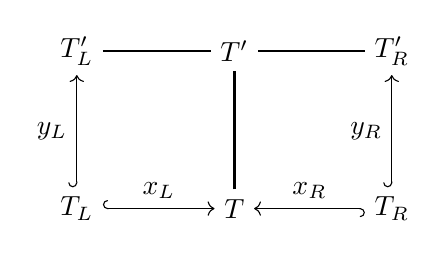
\begin{tikzpicture}
      \node (1) at (-2,1) {$T'_L$};
      \node (2) at (0,1) {$T'$};
      \node (3) at (2,1) {$T'_R$};
      \node (4) at (-2,-1) {$T_L$};
      \node (5) at (0,-1) {$T$};
      \node (6) at (2,-1) {$T_R$};
      \draw[right hook->] (4)--(5) node[midway,above] {$x_L$};
      \draw[right hook->] (6)--(5) node[midway,above] {$x_R$};
      \draw[right hook->] (4)--(1) node[midway,left] {$y_L$};
      \draw[right hook->] (6)--(3) node[midway,left] {$y_R$};
      \draw[thick] (1)--(2);
      \draw[thick] (3)--(2);
      \draw[very thick] (5)--(2);
    \end{tikzpicture}
    \caption{}
    \label{fig:DPjoinmap}
  \end{figure}

  In order to obtain $T'$ from $T$, we will essentially need to be able to reverse the
  reduction operation $T_H=\red(\rlstan{b_H}(T_H')$ that has been
  applied to $T_H'$ to obtain $T_H$ for every $H \in \{L,B\}$. To do
  so we will make use of the plug in operation.
    
  Our first order of business is to rename all forgotten features in
  $T$ to their real features as given by $T_L'$ and $T_R'$. That is,
  for every node $t$ in $T$ assigned to a forgotten feature, i.e.,
  $\feat_T(t) \in \SoFF{[k_L]}\cup\SoFF{[k_R]}$, we do the following.
  If $\feat_T(t) \in \SoFF{[k_H]}$ for $H\in \{L,R\}$, then $t$ is also
  in $T_H$ and hence also in $T_H'$. Therefore, we
  can change $\feat_T(t)$ to the real feature assigned to $t$ in
  $T_H'$. Let $T^0$ be the DT obtained from $T$ after renaming all
  forgotten features to real features in this manner.
  
  Consider an edge $e=(p,c)$ in $T_L$ such that $p$ is the parent of $c$
  in $T_L$. Then, $e$ corresponds to a path $P_L'(e)$ between
  $y_L(p)$ and $y_L(c)$ in $T_L'$. Similarly, $e$ corresponds to a
  path $P_L(e)$ between $x_L(p)$ and $x_L(c)$ in $T^0$.

  Our next order of business is now to add all nodes to $T^0$ that have been
  removed when going from $T_L'$ to $T_L$ (via the reduction
  $\red(\rlstan{b_L}(T_L'))$). To achieve this, we go over
  every edge $e=(p,c)$ of $T_L$ such that $p$ is the parent of $c$ in
  $T_L$ and plug in the path $P_L'(e)$ (from $T_L'$) into the last edge
  on the path $P_L(e)$ (from $T^0$). Let $T^1$ be the tree obtained from
  $T^0$ after doing this operation for every edge of $T_L$.

  Consider an edge $e=(p,c)$ in $T_R$ such that $p$ is the parent of $c$
  in $T_R$. Then, $e$ corresponds to a path $P_R'(e)$ between
  $y_R(p)$ and $y_R(c)$ in $T_R'$. Similarly, $e$ corresponds to a
  path $P_R(e)$ between $x_R(p)$ and $x_R(c)$ in $T^1$. 
  Similarly to above, we now add all nodes to $T^1$ that have been
  removed when going from $T_R'$ to $T_R$ (via the reduction
  $\red(\rlstan{b_R}(T_R'))$). To achieve this, we go over
  every edge $e=(p,c)$ of $T_R$ such that $p$ is the parent of $c$ in
  $T_R$ and plug in the path $P_R'(e)$ (from $T_R'$) into the last edge
  on the path $P_R(e)$ (from $T^1$). Let $T'$ be the tree obtained from
  $T^1$ after doing this operation for every edge of $T_R$.

  We now show that $T'$ is indeed a witness for the semi-validity of the record
  $(\hat{T},s_L+s_R+\hat{s})$, i.e., $T'$ is a reduced DT template for $b$
  such that
  $\hat{T}=\red(\rlstan{b}(T'))$ and $s_L+s_R+\hat{s}=|V(T')\setminus V(\hat{T})|$.

  We start by showing that $T'$ is reduced. First note that because
  $T$ is reduced so is $T^0$. Consider a node $t \in V(T')$. If
  $\feat_{T'}(t)\in \feat(b_H)$ for some $H \in \{L,R\}$, then $t$ is
  also in $V(T_H')$. Therefore, if $t$ were redundant in $T'$, it
  would also be redundant in $T_H'$, which cannot be the case because
  $T_H'$ is reduced. Moreover, if on the other hand, $\feat_{T'}(t)
  \in \SoIF{[k]}$, then $t$ is in $T^0$ and therefore cannot be
  redundant because $T^0$ is reduced. Therefore, $T'$ is reduced and
  it obviously only uses features in $\feat(b)\cup \SoFF{[k]}$. We
  show next that $T'$ is a DT template for $b$, i.e., $T'$ classifies all examples in
  $\exam(b)$ correctly. Towards showing this, let $e \in
  \exam(b)$, then $e \in \exam(b_H)$ for some $H\in
  \{L,R\}$. Because $T_H'$ is a DT template for $b_H$, we know that
  $e$ is correctly classified by $T_H'$. Let $\ell$ be the leaf in $T_H'$
  that contains $e$, i.e., $e \in E_{T_H'}(\ell)$ and let $Q$ be the path
  from the root of $T_H'$ to $\ell$. Then, $\ell$ also exists
  in $T'$ and moreover the path $P$ from the root of $T'$ to $\ell$
  contains all nodes of $Q$. Note furthermore that if a node $t$ in
  $Q$ has its left/right child on $Q$, then the same holds on $P$.
  We will show that $e$ follows
  along the path $P$ in $T'$ and therefore ends up in $\ell$, which shows
  that $e$ is correctly classified by $T'$.

  Let $t$ be a node of
  $P$. If $t$ is also in $Q$, then $e$ will be send to the child of
  $t$ in $P$. Otherwise, $t$ is either
  in $V(T)\setminus V(T_H)$ or $t$ is in $T_{\overline{H}}'\setminus
  T_{\overline{H}}$, where $\overline{H}=L$ if $H=R$ and
  $\overline{H}=R$ otherwise.
  
  In the former case, $\feat_{T'}(t) \in \SoIF{[k]}$ or $\feat_{T'}(t)
  \in \feat(b_{\overline{H}})$, which implies that $t$ behaves towards
  $e$ in the same manner as some future feature $f_{L} \in
  \SoIF{[k]}$, i.e., if $\feat_{T'}(t) \in \SoIF{[k]}$, then
  $f_L=\feat_{T'}(t)$ and if $\feat_{T'}(t)
  \in \feat(b_{\overline{H}})$, then $f_L=\rlL(\feat_T(t))$. Moreover,
  $t$ is redundant in $\rlL(T)$ because of its ancestors in $T_H$,
  i.e., either $A_{\rlL{T}}(t) \subseteq L $ or
  $A_{\rlL{T}}(t) \subseteq \overline{L}$. Because all these ancestors
  are in $T_H$ and therefore on $Q$, $\lab_{b_L}(e) \in
  A_{\rlL{T}}(t)$, which implies that $e$ is send to the non-redundant
  child of $t$. Finally, since $P$ contains $\ell$ it follows that $P$
  contains also the non-redundant child of $t$ in $\rlL(T)$ and
  therefore $e$ is send to the child of
  $t$ on $P$, as required. 
  
  In the latter case, i.e., the case that $t$ is in $V(T_{\overline{H}}')\setminus
  V(T_{\overline{H}})$, $t$ is redundant in
  $\rlstan{b_{\overline{H}}}(T_{\overline{H}}')$ because of some
  ancestor $t' \in V(T_{\overline{H}})$ with
  $\rlstan{b_{\overline{H}}}(\feat_{T'}(t))=\rlstan{b_{\overline{H}}}(\feat_{T'}(t'))$.
  Therefore, $\feat_{T'}(t')$ behaves in the same manner towards $e$
  as $\feat_{T'}(t)$, which because $t'$ is on $Q$ (because $t' \in
  V(T_{\overline{H}})$) implies that $e$ is
  send to the (non-redundant) child of $t$ on $P$.


  \newcommand{\rlTpT}{\alpha_{T'\rightarrow T}}
  It remains to show that $\hat{T}=\red(\rlstan{b}(T'))$ and
  $s_L+s_R+\hat{s}=|V(T')\setminus V(\hat{T})|$. Towards showing this,
  we first show that $T=\red(\rlTpT(T'))$, where $\rlTpT=\rltbiL \circ
  \rlstan{b_R} \circ \rltbiL \circ \rlstan{b_L}$. In other words, we
  need to show that the set of redundant nodes in $\rlTpT(T')$ is equal to
  $V(T')\setminus V(T)=V(T')\setminus V(T^0)$. Because, as shown above
  $T'$ is reduced, it follows that if a node $t$ is redundant
  $\rlTpT(T')$, then $t \in \feat_{T'}(b_H)$ for some $H
  \{L,R\}$. Because all such nodes, i.e., nodes $t$ in $T'$ with $t
  \in \feat_{T'}(b_H)$ are also in $T_H'$, we obtain that $t$ is
  redundant in $\rlTpT(T')$ if and only if it is redundant in
  $\rlstan{b_H}(T_H')$. Therefore, $\bigcup_{H \in
    \{L,R\}}V(T_H')\setminus V(T_H)$ is the set of all redundant nodes
  in $\rlTpT(T')$, which is equal to $V(T')\setminus V(T^0)$ by
  construction of $T'$, as required. Note that $|V(T')\setminus
  V(T^0)|=s_L+s_R$ because of the construction of $T'$. Now, because
  $\hat{T}=\red(\rltb(T))$ and $\rlstan{b}=\rltb \circ
  \rlTpT$, we obtain from Lemma~\ref{lem:frlred} that
  $\hat{T}=\red(\rlstan{b}(T'))$. Finally, because $|V(T')\setminus
  V(T^0)|=s_L+s_R$ and $|V(T^0)\setminus V(\hat{T})|=\hat{s}$, it
  follows that $|V(T')\setminus V(\hat{T})|=s_L+s_R+\hat{s}$, as required.
\end{proof}

\begin{lemma}[relabel node]\label{lem:relabel}
  Let $b\in V(B)$ be relabelling node in $B$. Then $\RRR(b)$ can be
  computed in time $\bigoh(2^{2k+1}\tfDTsenum)$.
\end{lemma}
\begin{proof}
  Let $c$ be the unique child of $b$ in $B$ and let $R_b : [k]
  \rightarrow [k]$ be the relabelling function associated with
  $b$. Because $B$ is nice, it holds that there are labels $i$ and $j$
  with $i \neq j$ such that $R(i)=j$ and $R(\ell)=\ell$ for every $\ell \in
  [k]\setminus \{i\}$.

  \newcommand{\g}{g}
  We say that a future feature $f_L \in \SoIF{[k]}$ is {\it good} if it does not
  distinguish between $i$ and $j$, i.e., $i\in L$ if and only if
  $j\in L$, and {\it bad} otherwise. For a bad future feature $f_L$,
  we denote by $\g(f_L)$ the good future feature $f_{\g(L)}$, where
  $\g(L)=L\cup \{i\}$ if $j \in L$ and $\g(L)=L\setminus \{i\}$,
  otherwise, i.e., informally, $g(f_L)$ is the good feature corresponding to $f_L$
  that sends all examples with label $i$ to the same side as $f_L$
  sends all examples with label $j$.
  

  \newcommand{\rlrelF}{\alpha^F_{i\rightarrow j}}
  \newcommand{\rlrelI}{\alpha^I_{i\rightarrow j}}
  To obtain the set $\RRR(b)$ of valid records for $b$, we first
  enumerate all reduced DT skeletons $T$ for $b$. Let $\rlrelI : \SoIF{[k]}
  \rightarrow \SoIF{[k]}$ be the function defined by setting
  $\rlrelI(f_L)=g(f_L)$ for every bad future feature $f_L \in
  \SoIF{[k]}$, i.e., $\rlrelI$ relabels every bad feature
  $f_L$ to its corresponding good feature $\g(f_L)$. Let
  $T^c=\red(\rlrelI(T))$. We now
  check whether $\RRR(c)$ contains a record of the form $(T^c,s^c)$. If
  not, then we disregard $T$. Otherwise, let $\rlrelF$ be the feature
  relabelling that relabels the forgotten feature $f_i$ to the
  forgotten feature $f_j$. Let $\hat{T}=\red(\rlrelF(T))$ and
  $\hat{s}=|V(T)\setminus V(\hat{T})|$. We now distinguish two
  cases. If we have not yet added any record of the form
  $(\hat{T},s')$ to $\RRR(b)$, then we add the record
  $(\hat{T},s^c+\hat{s})$ to $\RRR(b)$. Otherwise we replace the unique
  existing record $(\hat{T},s')$ with the record $(\hat{T},\min\{s',s^c+\hat{s}\})$.
  This completes the construction of the set
  $\RRR(b)$ of valid records. 

  Note that computing $\RRR(b)$ in this
  manner can be achieved in the stated run-time. This is because due
  to Corollary~\ref{cor:sizeofreduced} we can enumerate all possible
  choices for $T$ in time $\bigoh(\tfDTsenum)$ and for every such
  choice $T$ we can compute $T^c$ and $\hat{T}$ and check the existence of a record
  $(T^c,s)$ in $\RRR(c)$ in time at most
  $\bigoh(|T|)=\bigoh(2^{2k+1})$ (because of Corollary~\ref{cor:DTSsize}).

  It remains to show the correctness of our construction for $\RRR(b)$, i.e.,
  we have to show that a record is valid for $b$ if and only if we
  have added such a record according to our construction
  above. For this it suffices to show that a record is
  semi-valid for $b$ if and only if we have added such a record according to
  our construction above. This is because, a valid record $(T,s)$ can
  be obtained from the set of all semi-valid records $(T,s')$, where
  $s$ is the minimum $s'$ among all semi-valid records for $T$.

  Towards showing the forward direction, suppose that the record
  $(\hat{T},s)$ is semi-valid for $b$. Then, there is a reduced DT
  template $T'$ for $b$ such that $\hat{T}=\rlstan{b}(T')$ and
  $s=|V(T')\setminus V(\hat{T})|$. % now i need to get T^c', T, and T^c

  Let $T=\red(\rlstan{c}(T'))$. Then, $\hat{T}=\red(\rlrelF(T))$
  because of Lemma~\ref{lem:frlred} together with the observation that
  $\rlrelF \circ \rlstan{c}=\rlstan{b}$. Note that $T$ corresponds to the reduced
  DT skeleton considered by our construction. Let
  $T^c=\red(\rlrelI(T))$, let $\hat{s}=|V(T)\setminus V(\hat{T})|$,
  and let $s^c=s-\hat{s}$. It remains to show that the record $(T^c,s^c)$ is
  semi-valid for $c$. Let $T''=\red(\rlrelI(T'))$. Then, $T''$ is a
  reduced DT template for $c$, because so is $T'$ for $b$ and moreover
  all examples, in particular those with label $i$, in $\exam(c)$ end
  up in the same leaf in $T''$ as they do in $T'$; because of the
  relabelling $\rlrelI$ that relabelled all bad future features in
  $T'$ into their corresponding good future features in
  $T''$.
  Moreover, $T^c=\red(\rlstan{c}(T'')$ because of
  Lemma~\ref{lem:frlred} and furthermore
  $s^c=s-\hat{s}=|V(T'')\setminus V(T^c)|$. Therefore, $T''$ shows
  that $(T^c,s^c)$ is semi-valid for $c$.

  % $s=|V(T')\setminus V(\hat{T})|$
  % $s-\hat{s}=|V(T')\setminus V(T)|$
  
  Towards showing the reverse direction, suppose that we have added 
  the record $(\hat{T},s^c+\hat{s})$ using our construction. Then,
  there is a DT skeleton $T$ for $b$ with
  $\hat{T}=\red(\rlrelF(\hat{T}))$ and $\hat{s}=|V(T)\setminus
  V(\hat{T})|$ and a record $(T^c,s^c) \in \RRR(c)$ with
  $T^c=\red(\rlrelI(T))$.
  
  We have to show that the record $(\hat{T},s^c+\hat{s})$ is semi-valid for $b$. Because
  $(T^c,s^c) \in \RRR(c)$, there is a reduced DT template $T'$ for $c$ such that
  $T^c=\red(\rlstan{c}(T')$ and $s^c=|V(T')\setminus V(T^c)|$. 
  Informally, we now construct a witness $T'''$ for the semi-validity of $(\hat{T},
  s^c+\hat{s})$ for $b$ from $T'$ by reversing the reduction
  $T^c=\red(\rlrelI(T))$.

  Let $a : V(T^c) \rightarrow V(T')$ be the injective function that
  maps every node in $T^c$ to its corresponding node in $T'$; which
  exists because $T^c=\red(\rlstan{c}(T'))$. First 
  Let $b : V(T^c) \rightarrow V(T)$ be the injective function that
  maps every node in $T^c$ to its corresponding node in $T$; which
  exists because $T^c=\red(\rlrelI(T))$.
  First we relabel every future feature in $T'$ in to its
  corresponding future feature.
  Let $T''$ be the DT template obtained from $T'$ by setting
  $\feat_{T''}(a(b^{-1}(t)))=\feat_{T}(t)$ for every node $t \in
  V(T^c)$ with $\feat_T(t) \in \SoIF{[k]}$ and
  $\feat_{T''}(t)=\feat_{T'}(t)$ otherwise. Moreover, let $T'''$ be
  the DT template obtained from $T''$ by doing the following for every
  edge $e=(p,c)$ in $T^c$, where $p$ is the parent of $c$ in
  $T^c$. Let $P(e)$ be the path from $b(p)$ to $b(c)$ in $T$. Then, we
  plug in the path $P(e)$ into $T''$ at the edge $(p',a(c))$, where $p'$ is the
  parent of $a(c)$ in $T''$.
  \note{there is one problem remaining: $T'''$ could now have some
    forgotten features from $T$; those should be replaced by arbitrary
  real features with the same label; but only if such examples also
  exist; maybe there is a better way??}
  
  Then, $T'''$ is a DT template for $b$, because $T'$ is a DT template
  for $c$ and we only changed where examples with label $i$ go, which
  are not present in $\exam(b)$. Moreover, $T=\red(\rlstan{c}(T'''))$
  and therefore $\hat{T}=\red(\rlstan{b}(T''')$. Finally, because
  $|V(T''')\setminus V(T)|=|V(T')\setminus V(T^c)|=s^c$, it holds that
  $|V(T''')\setminus V(\hat{T})|=s^c+\hat{s}$, which shows that the
  record $(\hat{T},s^c+\hat{s})$ is semi-valid for $b$.
\end{proof}

We are now ready to proof the main result (Theorem~\ref{the:trac-nlcw-b-td}) of this
section.
\begin{proof}[Proof of Theorem~\ref{the:trac-nlcw-b-td}]
  Given $E$ and $B$, we use Lemmas~\ref{lem:leaf},~\ref{lem:join}, and~\ref{lem:relabel}
  to compute the set $\RRR(b)$ of valid records for every node $b$ of
  $B$ in a leaf-to-root manner. We then go through all records in
  $\RRR(r)$ for the root $r$ of $B$ to find a record
  $(T,s)$ such that $|V(T)|+s$ is minimum among all such records where
  $T$ is complete. The correctness of the algorithm follows directly
  from the definition of the valid records and
  Lemmas~\ref{lem:leaf},~\ref{lem:join}, and~\ref{lem:relabel}. Moreover, we obtain the
  run-time of the algorithm as follows.
  The maximum time spend on any of the
  nodes $b$ (which is achieved for a join-node) is
  $\bigoh(2^{3k+1}\tfDTsenumJN)$. Because $B$ has at most
  $\bigoh(k|E\cup \feat(E)|)$ nodes, we obtain
  $\bigoh(2^{3k+1}\tfDTsenumJN k|E\cup \feat(E)|)$ as the total
  run-time of the algorithm, which shows that \DTL{} is
  fixed-parameter tractable parameterized by the NLC-width (and
  therefore also the rank-width) of $E$.
\end{proof}

\section{Comparison with other Parameters}


\begin{proposition}\label{prop:rw-rrw}
Rank-width and renamable rank-width are domination-equivalent.  
\end{proposition}
\begin{proof}
  \newcommand{\comp}[2]{\textup{comp}(#1,#2)} Let $G$ be a bipartite
  graph with bipartition $(A,B)$ For a set $C \subseteq A\cup B$ the
  local bicomplement of $G$ w.r.t. $C$ is the bipartite graph
  $\comp{G}{C}$ with partition $(A,B)$ having an edge between
  $a \in A$ and $b\in B$ if either $\{a,b\}\setminus C\neq \emptyset$
  and $\{a,b\} \in E(G)$ or $\{a,b\} \subseteq C$ and
  $\{a,b\} \notin E(G)$. As observed by Kaminski et
  al.~\cite[Proposition~8]{KamiskiLM09}, the clique-width of
  $\comp{G}{S}$ and $G$ differ only by a constant factor. It is known
  that clique-width and rank-width of any graph can be mutually
  bounded by a function of each other. Consequently also the
  rank-width of $\comp{G}{S}$ and $G$ can be mutually be bounded by a
  function of each other. It remains to observe that for a CI $E$ and
  any renaming $E'=r_X(E)$, $G(E)$ is a local bicomplement of $G(E)$
  w.r.t.\ the set set $C=X\cup E$.
\end{proof}
\begin{proposition}\label{prop:rw-rtw}
Rank-width strictly dominates renamable treewidth.  
\end{proposition}
\begin{proof}
  Since for any graph $G$ we have $\rw(G) \leq \tw(G)+1$ \cite{Oum08},
  it follows that for CIs, renamable rank-width dominates renamable
  treewidth; hence, by Proposition~\ref{prop:rw-rrw}, rank-width
  dominates renamable treewidth. To show that the domination is
  strict, consider the CI $E_n$ with $4n$ features $f_i,g_i$,
  $1\leq i \leq 2n$, and $2n$ samples $e_j$, $1\leq j \leq 2n$.  We
  set $e_j(f_i)=0$ if $j\leq n$ and $e_j(f_i)=1$ otherwise, and we set
  $r_j(g_i)=1$ if and only if $i=j$.  The purpose of the $g_i$
  features is to keep any two examples distinct even if they agree on
  all the $f_i$ features.  Let $G_n$ be the graph obtained from
  $G(E_n)$ by deleting vertices of degree $\leq 1$; $G_n$ and $G(E_n)$
  have the same rank-width. Since $G_n$ is a complete bipartite it has
  constant rank-width; thus $G(E_n)$ has constant rank-width. However,
  for any $X\subseteq \feat(F)$, the graph $G(r_X(E_n))$ contains a
  $K_{n,n}$ as a subgraph, hence the renamable treewidth of $E_n$
  is~$n$.
\end{proof}
\begin{proposition}\label{prop:rtw-tw}
  Renamable treewidth strictly dominates treewidth.
\end{proposition}
\begin{proof}
  Domination follows by definition. To show that the domination is
  strict, consider the CI $E_n'$ obtained from the above CI $E_n$ by
  deleting the examples $e_{n+1},\dots,e_{2n}$ and the features
  $e_{n+1},\dots,e_{2n}$.  Since $G(E_n')$ contains $K_{n,n}$ as a
  subgraph, the treewidth of $E_n'$ is at least $n$. However, for
  $X=\{f_1,\dots,f_n\}$, the only edges of $G(r_X(E_n'))$ are of the
  form $\{e_i,g_i\}$, $1\leq i \leq n$, hence the renamable treewidth
  of $E_n'$ is constant.
\end{proof}




\section{Conclusion}
We have initiated the study of the parameterized complexity of learning DTs from data. Our main tractability result provides novel insights into the structure of DTs and is based on the NLC-width parameter that seems to be well suited to measure the complexity of input instances for the problem.

The problem of learning DTs comes in many variants and flavors, which opens up a wide range of new research directions to explore. For instance:

\begin{itemize}
\item What other (structural) parameters can be exploited to
  efficiently learn DTs? Is learning DTs of small size fixed-parameter
  tractable parameterized by the rank-width of $G(E)$?
\item Instead of learning DTs of small size, one often wants to learn DTs of small height. Therefore, it is natural to ask whether our approach can be also used in this setting. While one can adapt our approach to obtain an XP-algorithm for learning DTs of small height parameterized by NLC-width, it is not clear to us whether the problem also allows for an fpt-algorithm. 
\item Can we extend our approach to CIs, where features range over an arbitrary domain? In this case, one usually still uses DTs that make binary decisions (i.e. whether a feature is smaller equal or larger than a given threshold). While it is relatively easy to see that our approach can be extended if the  domain's size (for every feature) is bounded or used as an additional parameter, it is not clear what happens if the size of the domain is allowed to grow arbitrarily.
\end{itemize}

\bibliography{literature}
\end{document}
%%% Local Variables:
%%% mode: latex
%%% TeX-master: t
%%% End:
